В данной главе рассматривается задача выбора моделей глубокого обучения субоптимальной сложности. Под сложностью модели понимается правдоподобие модели~\eqref{eq:evidence}. Под субоптимальной сложностью понимается приближенная оценка правдоподобия модели, полученная с использованием вариационных методов. Вводятся вероятностные предположения о распределении параметров. На основе байесовского вывода предлагается функция правдоподобия модели. Для получения оценки правдоподобия применяются вариационные методы с использованием градиентных алгоритмов оптимизации. Проводится вычислительный эксперимент на нескольких выборках.

В данной работе предлагается метод получения вариационной нижней оценки  правдоподобия модели с использованием модифицированного алгоритма стохастического градиентного спуска. {Модификация заключается в добавлении шумовой компоненты. Эта компонента позволяет получить более точные оценки правдоподобия модели для сравнения моделей и выбора наиболее адекватной из них. } Рассматривается ряд модификаций базового алгоритма. {В качестве базового алгоритма выступает алгоритм оптимизации параметров модели с использованием стохастического градиентного спуска без контроля переобучения. Он заключается в итеративном вычислении градиента по параметрам от функции правдоподобия обучающей выборки и изменении значений параметров с его учетом.} Приводится сравнение с алгоритмом получения вариационной нижней оценки, представленном в~\cite{nips}. {Рассматриваются следующие модификации базового алгоритма:
%\begin{enumerate}
%\item 
оптимизация с кросс-валидацией с использованием и без использования регуляризации модели,
алгоритм получения вариационной оценки правдоподобия модели с применением нормального распределения,
алгоритм получения вариационной оценки правдоподобия с использованием стохастического градиентного спуска,
алгоритм получения вариационной оценки правдоподобия с использованием стохастической динамики Ланжевена.}
 { Данные алгоритмы решают следующие проблемы оптимизации моделей  градиентным спуском: оптимизация модели с меньшими затратами вычислительных ресурсов, быстрая сходимость оптимизации, контроль переобучения и выбор наиболее адекватной модели.
Под переобучением понимается потеря обобщающей способности модели с увеличением правдоподобия обучающей выборки~\cite{MacKay}. Переобучение характерно для моделей с большим количеством параметров, сопоставимым с мощностью обучающей выборки, что встречается в случае выбора моделей глубокого обучения~\cite{hinton_rbm, suts}.
}
Также алгоритмы имеют дальнейшую возможность применения к градиентным алгоритмам оптимизации гиперпараметров, описанным в~\cite{hyper}.

Свойства представленных в данной работе  алгоритмов исследуется на выборках, на которых проверялась работа алгоритма вероятностного обратного распространения ошибок~\cite{pbp}, где авторы акцентируются на оптимизации параметров модели. 


\section{Постановка задачи оптимизации правдоподобия моделей}
Определим понятие статистической сложности модели. Сложностью модели будем называть \textit{правдоподобие модели}~\eqref{eq:evidence}.
Пусть задано множество моделей $M$, для которых, возможно, не определена общая параметризация.
Для каждой модели $\mathbf{f} \in {M}$ заданы различные значения гиперпараметров $\mathbf{h}$. 
Рассмотрим два подхода к сравнению сложностей моделей:
\begin{enumerate}
\item Модели $\mathbf{f}$ принадлежат одному семейству $\mathfrak{F}$. При таком подходе сравнение сложности различных моделей является  адекватным, т.к. они определены на общем пространстве структур $\amsmathbb{\Gamma}$ и параметров $\mathbb{W}$. Недостатком такого подхода является сложность вычисления правдоподобия модели в случае, когда структура $\boldsymbol{\Gamma}$ определена однозначно, что может противоречить введенным вероятностным предположениям о структуре модели.
\item Модели $\mathbf{f}$  рассматриваются независимо от общей параметризации. Недостатком такого подхода является возможная некорректность сравнения моделей с заведомо различными структурами моделей, сильно отличающимися по количеству параметров. Возможным решение данного недостатка является введение дополнительного штрафа за большое количество параметров в модели~\cite{MacKay}.
\end{enumerate}
В данном разделе рассматривается второй вариант. Будем полгать, что структура модели $\boldsymbol{\Gamma}$ для вероятностной модели глубокого обучения $\mathbf{f}$ определена однозначно. Тем не менее, основная часть данной главы также применима и ко первому варианту.

\begin{defin} Сложностью модели $\mathbf{f}$ назовем правдоподобие модели:
\begin{equation}
\label{eq:model_evidence}
	p(\mathbf{y}|\mathbf{X},\mathbf{h}) = \int_{\mathbf{w} \in \mathbb{W}} p(\mathbf{y}|\mathbf{X},\mathbf{w}, \mathbf{h})p(\mathbf{w}|\mathbf{h})d\mathbf{w}.
\end{equation}
\end{defin}


\begin{defin}Модель классификации $\mathbf{f}$ назовем оптимальной среди моделей $M$, если достигается максимум интеграла~\eqref{eq:model_evidence}.
\end{defin}


Требуется найти оптимальную модель $\mathbf{f}$ из заданного множества моделей $M$, а также значения ее параметров $\mathbf{w}$, доставляющие максимум апостериорной вероятности
\begin{equation}
\label{eq:var_inf_posterior}
	p(\mathbf{w}|\mathbf{y},\mathbf{X},\mathbf{h}) = \frac{p(\mathbf{y}|\mathbf{X}, \mathbf{w}, \mathbf{h})p(\mathbf{w}|\mathbf{h})}{p(\mathbf{y}|\mathbf{X}, \mathbf{h})}.
\end{equation}


%\begin{example_empty}
\begin{example}
Рассмотрим задачу линейной регрессии:
\[
	\mathbf{y} =\mathbf{X} \mathbf{w} + \boldsymbol{\varepsilon},\quad \boldsymbol{\varepsilon}  \sim \mathcal{N}(\mathbf{0},\mathbf{1}),\quad \mathbf{w} \sim  \mathcal{N}(\mathbf{0},\mathbf{A}^{-1}),
\]
где $\mathbf{A}$ --- диагональная матрица. 
Правдоподобие зависимой переменной имеет вид
\begin{equation}
\label{eq:example1}
	p(\mathbf{y}|  \mathbf{X}, \mathbf{w}, \mathbf{h}) = (2\pi) ^{-\frac{m}{2}} \textnormal{exp} \bigl(-\frac{1}{2}(\mathbf{y} -\mathbf{X} \mathbf{w})^\mathsf{T}(\mathbf{y} - \mathbf{X}\mathbf{w})\bigr),
\end{equation}
априорное распределение параметров модели имеет вид
\begin{equation}
\label{eq:prior}	
p(\mathbf{w}|\mathbf{h}) =  (2\pi) ^{-\frac{n}{2}} |\mathbf{A}|^{\frac{1}{2}} \textnormal{exp} (-\frac{1}{2}\mathbf{w}^\mathsf{T}\mathbf{A}\mathbf{w}).
\end{equation}

Правдоподобие модели~\eqref{eq:evidence} в этом примере вычисляется аналитически~\cite{hyperopt}:
\begin{equation}
\label{eq:ground}
	p(\mathbf{y}|\mathbf{X},\mathbf{h})  =  (2\pi) ^{-\frac{m}{2}} |\mathbf{A}|^{\frac{1}{2}} |\mathbf{H}|^{-\frac{1}{2}}  \textnormal{exp}\bigl(-\frac{1}{2}(\mathbf{y} -\mathbf{X} \hat{\mathbf{w}})^\mathsf{T}(\mathbf{y} - \mathbf{X}\hat{\mathbf{w}})\bigr)\textnormal{exp} \bigl(-\frac{1}{2}\hat{\mathbf{w}}^\mathsf{T}\mathbf{A}\hat{\mathbf{w}}\bigr),
\end{equation}
где $\hat{\mathbf{w}}$ --- значение наиболее вероятных~\eqref{eq:posterior} параметров модели:
\[
	\hat{\mathbf{w}} = \argmax p(\mathbf{w}|\mathbf{y}, \mathbf{X}, \mathbf{h}) = (\mathbf{A} + \mathbf{X}^\mathsf{T}\mathbf{X})^{-1}\mathbf{X}^\mathsf{T}\mathbf{y},
\]
$\mathbf{H}$ --- гессиан функции потерь $L$ модели:
\[
	\mathbf{H}	= \nabla \nabla_\mathbf{w} \left(\frac{1}{2} (\mathbf{y} -\mathbf{X} {\mathbf{w}})^\mathsf{T}(\mathbf{y} - \mathbf{X}{\mathbf{w}}) + \frac{1}{2}\mathbf{w}^\mathsf{T}\mathbf{A}\mathbf{w} \right) = \mathbf{A} + \mathbf{X}^\mathsf{T}\mathbf{X},
\]

\[ 
	L = - \textnormal{log} p(\mathbf{y}|  \mathbf{X}, \mathbf{w}, \mathbf{h}). 
\]
\end{example}

\begin{example}
Рассмотрим задачу классификации, в которой модель --- нейросеть с softmax-слоем на выходе:
\[
\mathbf{f} = \mathbf{f}_\textnormal{|V|}(\mathbf{f}_{|V|-1}(\dots \mathbf{f}_1(\mathbf{x}))),
\]
$\mathbf{f}_1, \dots, \mathbf{f}_|V|$ --- дифференцируемые функции, $\mathbf{f}_\textnormal{|V|}$ --- многомерная логистическая функция:
\[
	\mathbf{f}_\textnormal{|V|} = \frac{\mathbf{f}_{|V|-1}(\dots \mathbf{f}_1(\mathbf{x}))}{\sum_{r=1}^Z \textnormal{exp}\bigl( {f}^{r}_{|V|-1}(\dots \mathbf{f}_1(\mathbf{x})) \bigr)},
\]
где ${f}_{|V|-1}^{r}$ --- $r$-я компонента функции $\mathbf{f}_{|V|-1}$. Компонента $r$ вектора $\mathbf{f}_{|V|}$ определяет вероятность принадлежности объекта $\mathbf{x}$ к классу $r$. Логарифм правдоподобия зависимой переменной аналогично~\eqref{eq:example1} имеет вид
\[
	\textnormal{log} p({y}|\mathbf{x}, \mathbf{w}, \mathbf{h}) =  \textnormal{log}~{f}^{y}_{|V|} (\mathbf{f}_{|V-1|}(\dots \mathbf{f}_1(\mathbf{x}))).
\]

Данная модель описывает многослойную сеть, аналогичную моделям семейства, представленного на Рис.~\ref{fig:scheme_mlp}.
\end{example}

Интеграл правдоподобия~\eqref{eq:model_evidence} модели является трудновычислимым для данного семейства моделей. Одним из методов вычисления приближенного значения правдоподобия является получение вариационной оценки правдоподобия.  


{В качестве функции, приближающей логарифм интеграла~\eqref{eq:model_evidence}, будем рассматривать его нижнюю оценку, полученную при помощи неравенства Йенсена~\cite{Bishop}. Получим нижнюю оценку логарифма правдоподобия модели, используя неравенство}
\begin{equation} 
\label{eq:var_elbo}
\textnormal{log}~p(\mathbf{y}|\mathbf{X},\mathbf{h})  = \int_{\mathbf{w}} q(\mathbf{w})\textnormal{log}~\frac{p(\mathbf{y},\mathbf{w}|\mathbf{X},\mathbf{h})}{q(\mathbf{w})}d\mathbf{w} + \textnormal{D}_\textnormal{KL}  \bigl(q(\mathbf{w})||p(\mathbf{w}|\mathbf{y}, \mathbf{X}, \mathbf{h})\bigr) \geq	
\end{equation} 
$$
\geq \int_{\mathbf{w}} q(\mathbf{w})\textnormal{log}~\frac{p(\mathbf{y},\mathbf{w}|\mathbf{X},\mathbf{h})}{q(\mathbf{w})}d\mathbf{w} =
$$

$$
= -\textnormal{D}_\textnormal{KL} \bigl(q(\mathbf{w})||p(\mathbf{w}|\mathbf{h})\bigr) + \int_{\mathbf{w}} q(\mathbf{w})\textnormal{log}~{p(\mathbf{y}|\mathbf{X},\mathbf{w},\mathbf{h})} d \mathbf{w},
$$
где $\textnormal{D}_\textnormal{KL}\bigl(q(\mathbf{w})||p(\mathbf{w} |\mathbf{h})\bigr)$ --- расстояние Кульбака--Лейблера между двумя распределениями: $$\textnormal{D}_\textnormal{KL}\bigl(q(\mathbf{w})||p(\mathbf{w} |\mathbf{h})\bigr) = -\int_{\mathbf{w}} q(\mathbf{w})\textnormal{log}~\frac{p(\mathbf{w} | \mathbf{h})}{q(\mathbf{w})}d\mathbf{w},$$
$$
p(\mathbf{y},\mathbf{w}|\mathbf{X},\mathbf{h}) = p(\mathbf{y}|\mathbf{X},\mathbf{h})p(\mathbf{w}|\mathbf{h}).
$$

{
\begin{defin} Вариационной оценкой логарифма правдоподобия модели~\eqref{eq:model_evidence} $\textnormal{log}~p(\mathbf{y}|\mathbf{X},\mathbf{h})$ называется оценка $\textnormal{log}~\hat{p}(\mathbf{y}|\mathbf{X},\mathbf{h})$, полученная аппроксимацией неизвестного апостериорного распределения $p(\mathbf{w}| \mathbf{y}, \mathbf{X}, \mathbf{h})$ заданным распределением $q(\mathbf{w})$.
\end{defin}
}


Будем рассматривать задачу нахождения вариационной оценки как задачу оптимизации. Пусть задано множество распределений $\mathfrak{Q} =\{q(\mathbf{w})\}$. Сведем задачу нахождения наиболее близкой вариационной нижней оценки интеграла~\eqref{eq:evidence} к оптимизации вида
\[
     \hat{q}(\mathbf{w}) = \argmax_{q \in \mathfrak{Q}}  \int_{\mathbf{w}} q(\mathbf{w})\textnormal{log}~\frac{p(\mathbf{y},\mathbf{w}|\mathbf{X},\mathbf{h})}{q(\mathbf{w})}d\mathbf{w}.
\]  
В данной работе в качестве множества $\mathfrak{Q}$ рассматривается нормальное распределение и распределение параметров, неявно получаемое оптимизацией градиентными методами. 

Оценка~\eqref{eq:var_elbo} является нижней, поэтому может давать некорректные оценки для правдоподобия~\eqref{eq:model_evidence}. Для того, чтобы оценить величину этой ошибки, докажем следующее утверждение.

\begin{theorem}[~\cite{Bishop}]\label{st:st1} Пусть задано множество $\mathfrak{Q} = \{q(\mathbf{w})\}$ непрерывных распределений. Максимизация вариационной нижней оценки $$\int_{\mathbf{w}} q(\mathbf{w})\textnormal{log}~\frac{p(\mathbf{y},\mathbf{w}|\mathbf{X},\mathbf{h})}{q(\mathbf{w})}d\mathbf{w}$$  логарифма интеграла~\eqref{eq:evidence}  эквивалентна минимизации расстояния Кульбака--Лейблера между распределением $q(\mathbf{w}) \in \mathfrak{Q}$ и апостериорным распределением параметров $p(\mathbf{w}|\mathbf{y}, \mathbf{X}, \mathbf{h})$:
\begin{equation}
\label{eq:optim}
    \hat{q} = \argmax_{q \in Q} \int_{\mathbf{w}} q(\mathbf{w})\textnormal{log}~\frac{p(\mathbf{y},\mathbf{w}|\mathbf{X},\mathbf{h})}{q(\mathbf{w})}d\mathbf{w} \Leftrightarrow 	
    \hat{q} = \argmin_{q \in Q} \textnormal{D}_\textnormal{KL}  \bigl(q(\mathbf{w})||p(\mathbf{w}|\mathbf{y}, \mathbf{X}, \mathbf{h})\bigr),
\end{equation}

\[
	\textnormal{D}_\textnormal{KL}  \bigl(q(\mathbf{w})||p(\mathbf{w}|\mathbf{y}, \mathbf{X}, \mathbf{h})\bigr) =  \int_\mathbf{w} q(\mathbf{w}) \frac{q(\mathbf{w})}{p(\mathbf{w}|\mathbf{y}, \mathbf{X}, \mathbf{h})} d\mathbf{w}.
\]

\end{theorem}
\begin{proof}
Доказательство непосредственно следует из~\eqref{eq:var_elbo}. Вычитая из обеих частей равенства $\textnormal{D}_\textnormal{KL}  (q(\mathbf{w})||p(\mathbf{w}|\mathbf{y}, \mathbf{X}, \mathbf{h}))$, получим
\[
\textnormal{log}~p(\mathbf{y}|\mathbf{X},\mathbf{h}) - \textnormal{D}_\textnormal{KL}  (q(\mathbf{w})||p(\mathbf{w}|\mathbf{y}, \mathbf{X}, \mathbf{h}))  = \int_{\mathbf{w}} q(\mathbf{w})\textnormal{log}~\frac{p(\mathbf{y},\mathbf{w}|\mathbf{X},\mathbf{h})}{q(\mathbf{w})}d\mathbf{w},
\]
где $\textnormal{log}~p(\mathbf{y}|\mathbf{X},\mathbf{h})$ --- выражение, не зависящее от $q(\mathbf{w})$.
\end{proof}



Таким образом, задача нахождения вариационной оценки, близкой к значению интеграла~\eqref{eq:model_evidence} сводится к поиску распределения $\hat{q}$, аппроксимирующего распределение $p(\mathbf{w}|\mathbf{y}, \mathbf{X}, \mathbf{h})$ наилучшим образом. 

\begin{defin} Пусть задано множество распределений $\mathfrak{Q}$. Модель $\mathbf{f}$ назовем субоптимальной на множестве моделей $M$, если модель доставляет максимум нижней вариационной оценке интеграла~\eqref{eq:optim}
\begin{equation}
\label{eq:var_elbo2}
	\max_{q \in \mathfrak{Q}}\int_{\mathbf{w}} q(\mathbf{w})\textnormal{log}~\frac{p(\mathbf{y},\mathbf{w}|\mathbf{X},\mathbf{h})}{q(\mathbf{w})}d\mathbf{w}.
\end{equation}
\end{defin}

{
Субоптимальность модели может быть также названа вариационной оптимальностью модели или LB-оптимальностью (\textit{Lower Bound --- нижняя граница}) модели.}

Вариационная оценка~\eqref{eq:var_elbo} интерпретируется как оценка сложности модели по принципу минимальной длины описания~\eqref{eq:mdl}, где первое слагаемое определяет количество информации для описания выборки, а второе слагаемое --- длину описания самой модели~\cite{nips}.

В данной работе решается задача выбора субоптимальной модели при различных заданных множествах $\mathfrak{Q}$.

\section{Методы получения вариационной оценки правдоподобия}
Ниже представлены методы получения вариационных нижних оценок~\eqref{eq:var_elbo2} правдоподобия~\eqref{eq:evidence}. В первом параграфе рассматривается метод, основанный на аппроксимации апостериорного распределения $p( \mathbf{w}|\mathbf{y}, \mathbf{X}, \mathbf{h})$~\eqref{eq:posterior} многомерным гауссовым распределением с диагональной матрицей ковариаций. В последующих параграфах рассматриваются методы, основанные на различных модификациях стохастического градиентного спуска. 

\textbf{Аппроксимация нормальным распределением. }
В качестве множества $\mathfrak{Q} = \{q(\mathbf{w})\}$ задано параметрическое семейство нормальных распределений с диагональными матрицами ковариаций:
\begin{equation}
\label{eq:diag}
	q \sim \mathcal{N}(\boldsymbol{\mu}_q, \mathbf{A}^{-1}_q),\quad,\boldsymbol{\theta}=[\boldsymbol{\mu}_q, \textbf{diag}(\mathbf{A}^{-1}_q)]
\end{equation}
где $\mathbf{A}_q$ --- диагональная матрица ковариаций, $\boldsymbol{\mu}_q$ --- вектор средних компонент.

Пусть априорное распределение $p(\mathbf{w}|\mathbf{h})$~\eqref{eq:prior} параметров модели задано как нормальное:
\[
	p(\mathbf{w}|\mathbf{h}) \sim \mathcal{N}(\boldsymbol{\mu}, \mathbf{A}^{-1}),\quad \mathbf{h} = \textbf{diag}(\mathbf{A}^{-1}_q),
\] 
Тогда оптимизация~\eqref{eq:optim} имеет вид
\begin{equation}
\label{eq:norm_max}
 \int_{\mathbf{w}} q(\mathbf{w})\textnormal{log}~{p(\mathbf{y}|\mathbf{X},\mathbf{w},\mathbf{h})} d \mathbf{w} - D_\textnormal{KL}\bigl(q (\mathbf{w} )|| p (\mathbf{w}|\mathbf{h})\bigr) \to \max_{\mathbf{A}_q, \boldsymbol{\mu}_q},
\end{equation}
где расстояние $D_\textnormal{KL}$ между двумя гауссовыми величинами рассчитывается как 
\[
	D_\textnormal{KL}\bigl(q (\mathbf{w}) || p (\mathbf{w}|\mathbf{h})\bigr) = \frac{1}{2} \bigl( \textnormal{Tr} [\mathbf{A}\mathbf{A}^{-1}_q] + (\boldsymbol{\mu} - \boldsymbol{\mu}_q)^\mathsf{T}\mathbf{A}(\boldsymbol{\mu} - \boldsymbol{\mu}_q) - u +\textnormal{ln}~|\mathbf{A}^{-1}| - \textnormal{ln}~|\mathbf{A}_q^{-1}| \bigr).
\]
В качестве приближенного значения интеграла $$\int_{\mathbf{w}} q(\mathbf{w})\textnormal{log}~{p(\mathbf{y}|\mathbf{X},\mathbf{w},\mathbf{h})} d \mathbf{w}$$ предлагается использовать формулу
\[
\int_{\mathbf{w}} q(\mathbf{w})\textnormal{log}~{p(\mathbf{y}|\mathbf{X},\mathbf{w},\mathbf{h})} d \mathbf{w} \approx \sum_{i=1}^m \textnormal{log}~p({y}_i|\mathbf{x}_i, \mathbf{w}_i),
\]
где $\mathbf{w}_i$  --- реализация случайной величины из распределения $q(\mathbf{w})$.

Итоговая функция оптимизации~\eqref{eq:norm_max} имеет вид
\begin{equation}
\label{eq:gaus}
	\mathbf{f} = \argmax_{\mathbf{A}_q, \boldsymbol{\mu}_q} \sum_{i=1}^m \textnormal{log}~p({y}_i|\mathbf{x}_i, \mathbf{w}_i) - D_\textnormal{KL}\bigl(q (\mathbf{w} )|| p (\mathbf{w}|\mathbf{h})\bigr).
\end{equation}

%\begin{example_empty} 
%\hspace{\parindent}
\begin{example}
Пусть  задана выборка $\mathfrak{D}$, в которой переменная ${y}$ не зависит от $\mathbf{x}$:
\begin{equation}
\label{eq:example_post}
	{y} \sim \mathcal{N}(\mathbf{w}, \mathbf{B}^{-1}),
\end{equation}

\[
	\mathbf{B}^{-1} = \left( \begin{array}{cc}
	2 & 1,8 \\
	1,8 & 2\\
	\end{array}  \right),
\]
\[
	p(\mathbf{w}|\mathbf{h}) = \mathcal{N}(\mathbf{0}, \mathbf{I}).
\]

График аппроксимации распределения параметров представлен на рис.~\ref{fig:var},\textit{а}. Как видно из графика, с использованием метода~\eqref{eq:gaus} получено грубое приближение апостериорного распределения $p(\mathbf{w}|\mathbf{y}, \mathbf{X}, \mathbf{h})$, что может существенно занизить оценку правдоподобия модели.


\begin{figure}[tbh!]



\minipage{0.32\textwidth}
 \caption*{\textit{а}}
  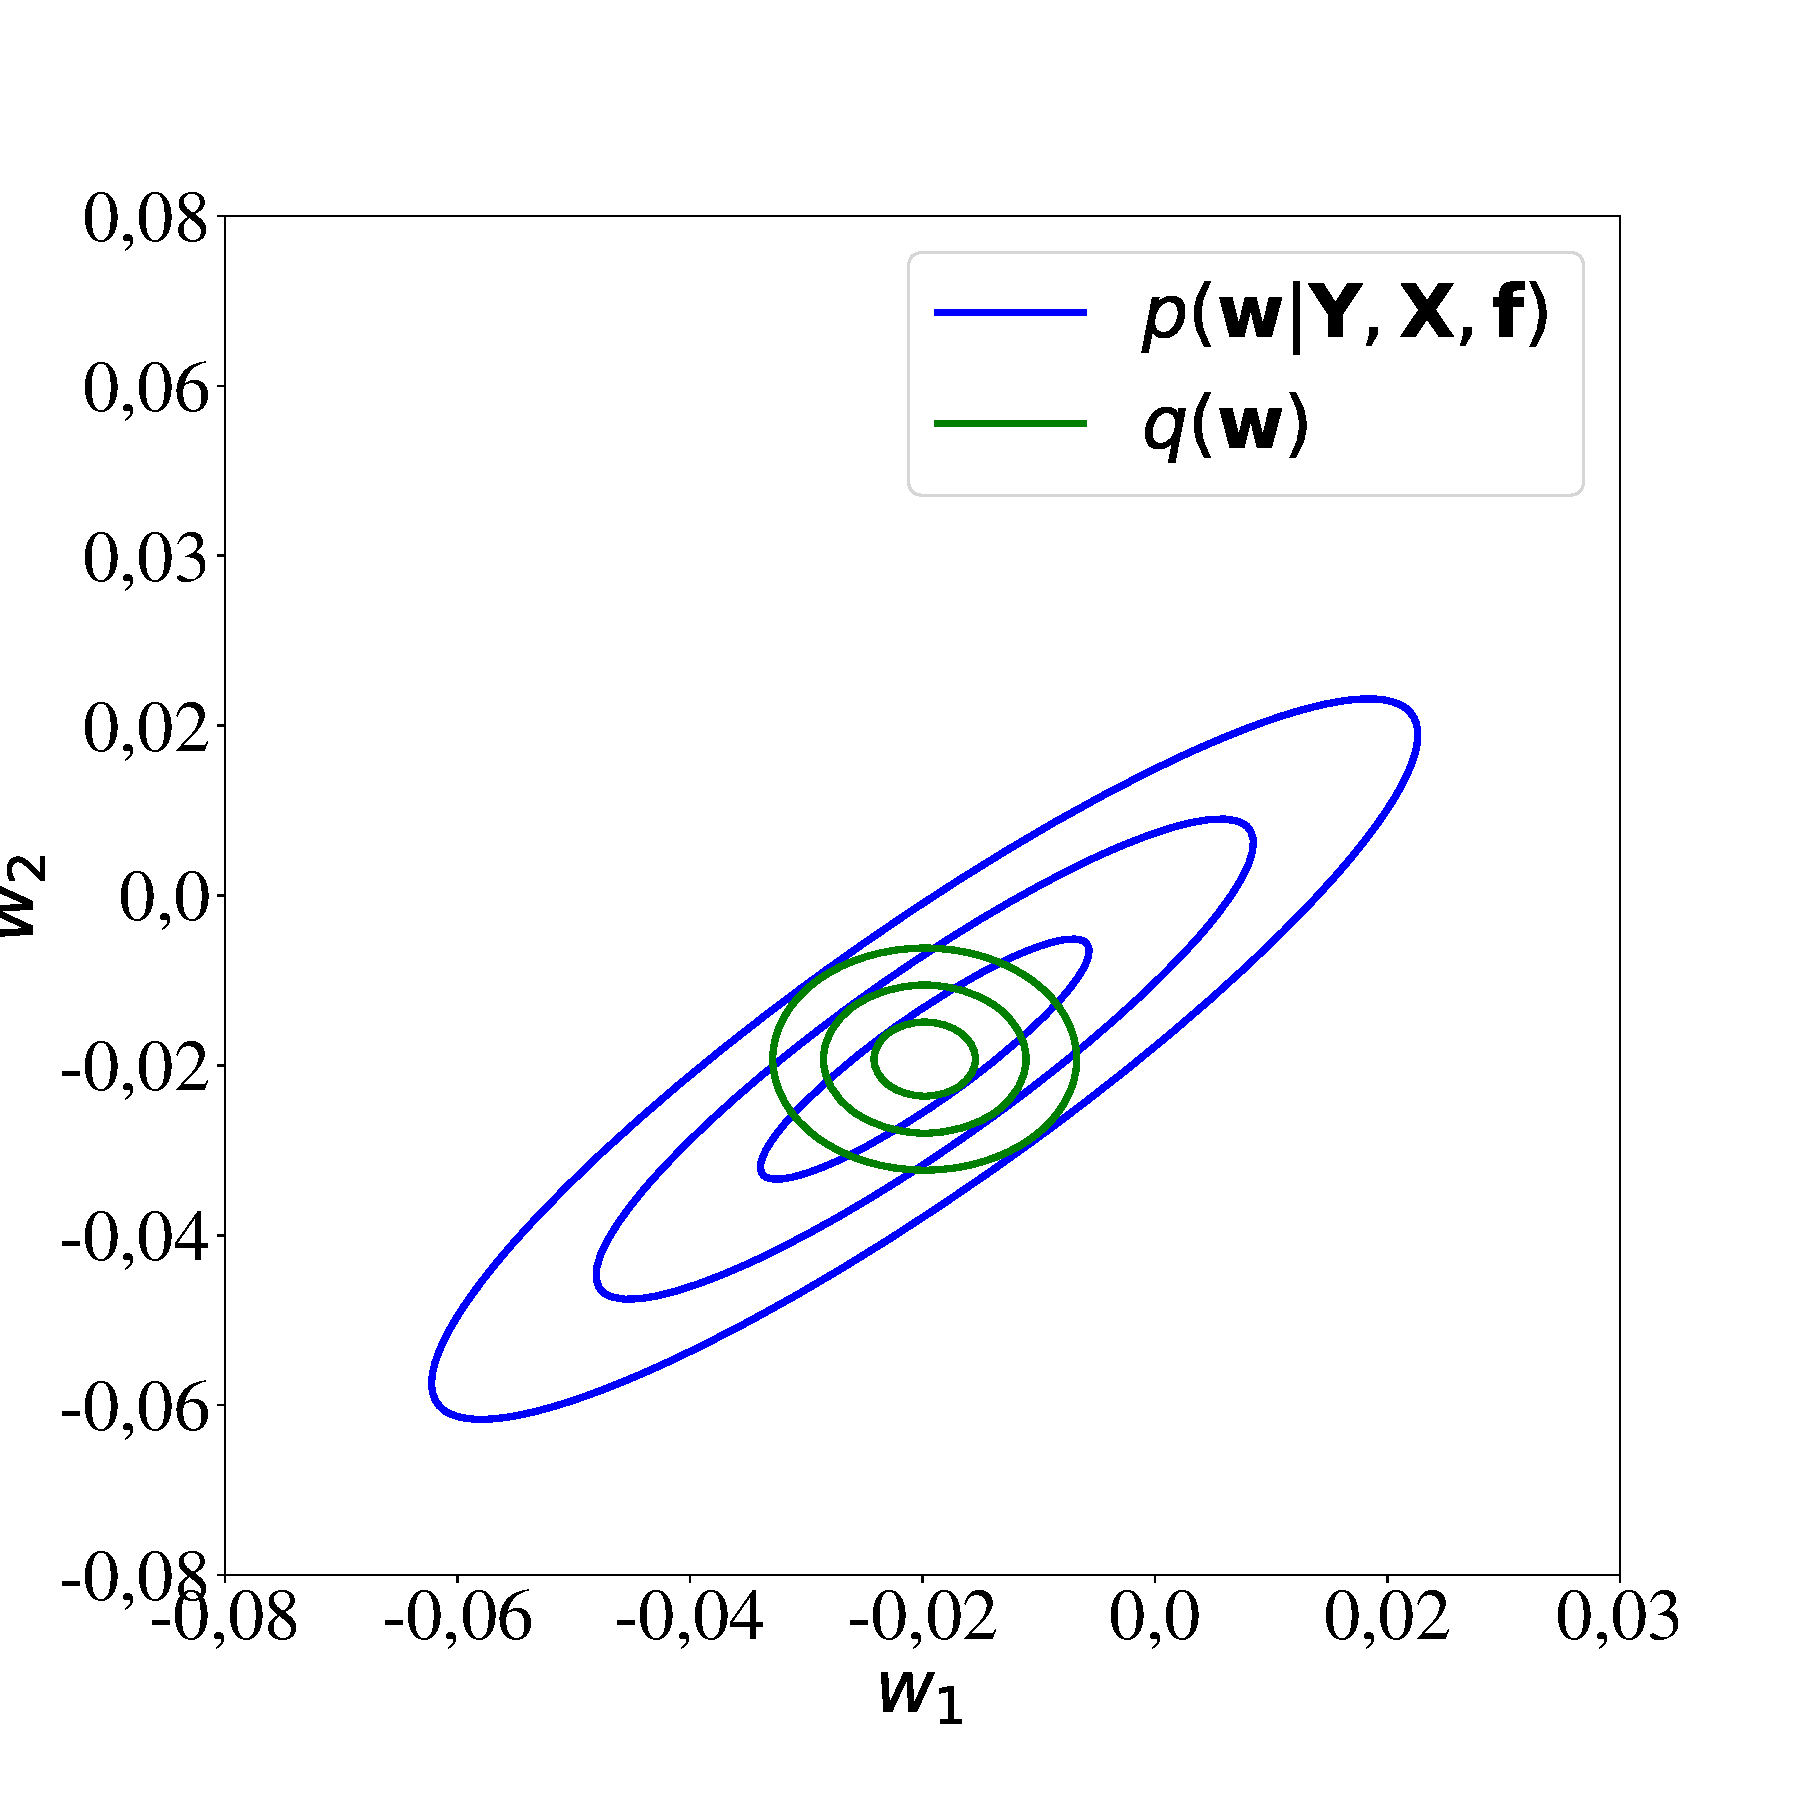
\includegraphics[width=\linewidth]{./plots/var/mf.pdf}

\endminipage\hfill
\minipage{0.32\textwidth}
\caption*{\textit{б}}
 
  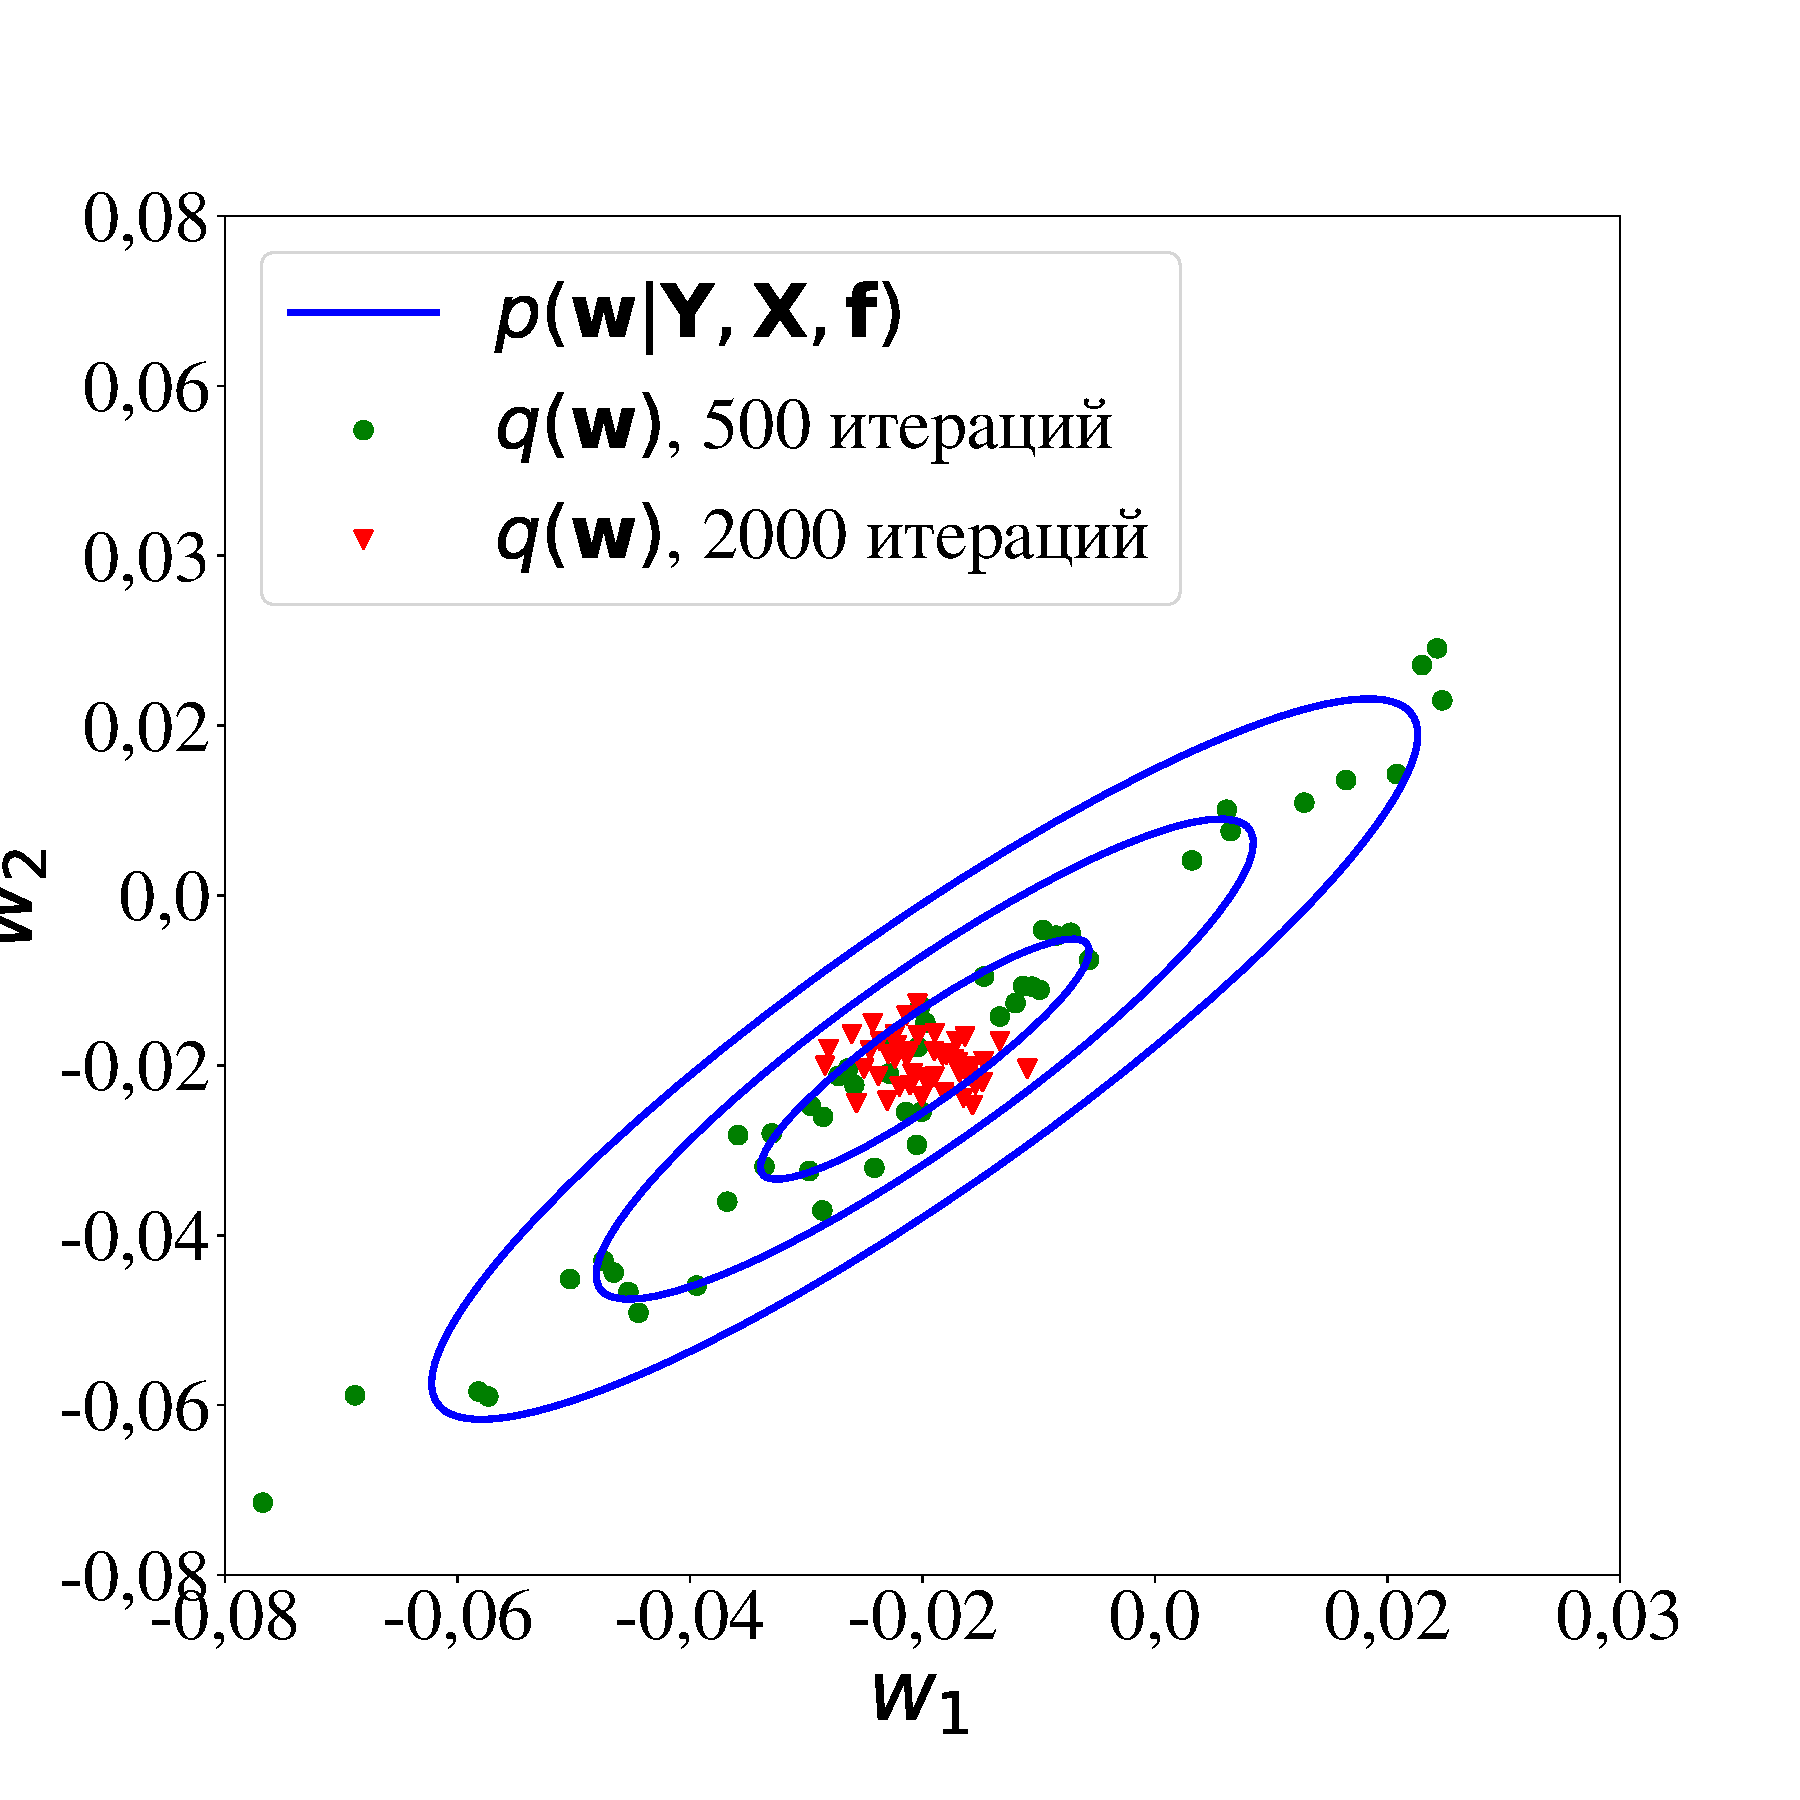
\includegraphics[width=\linewidth]{./plots/var/sgd.pdf}
 \endminipage\hfill
\minipage{0.32\textwidth}%
 \caption*{\textit{в}}

  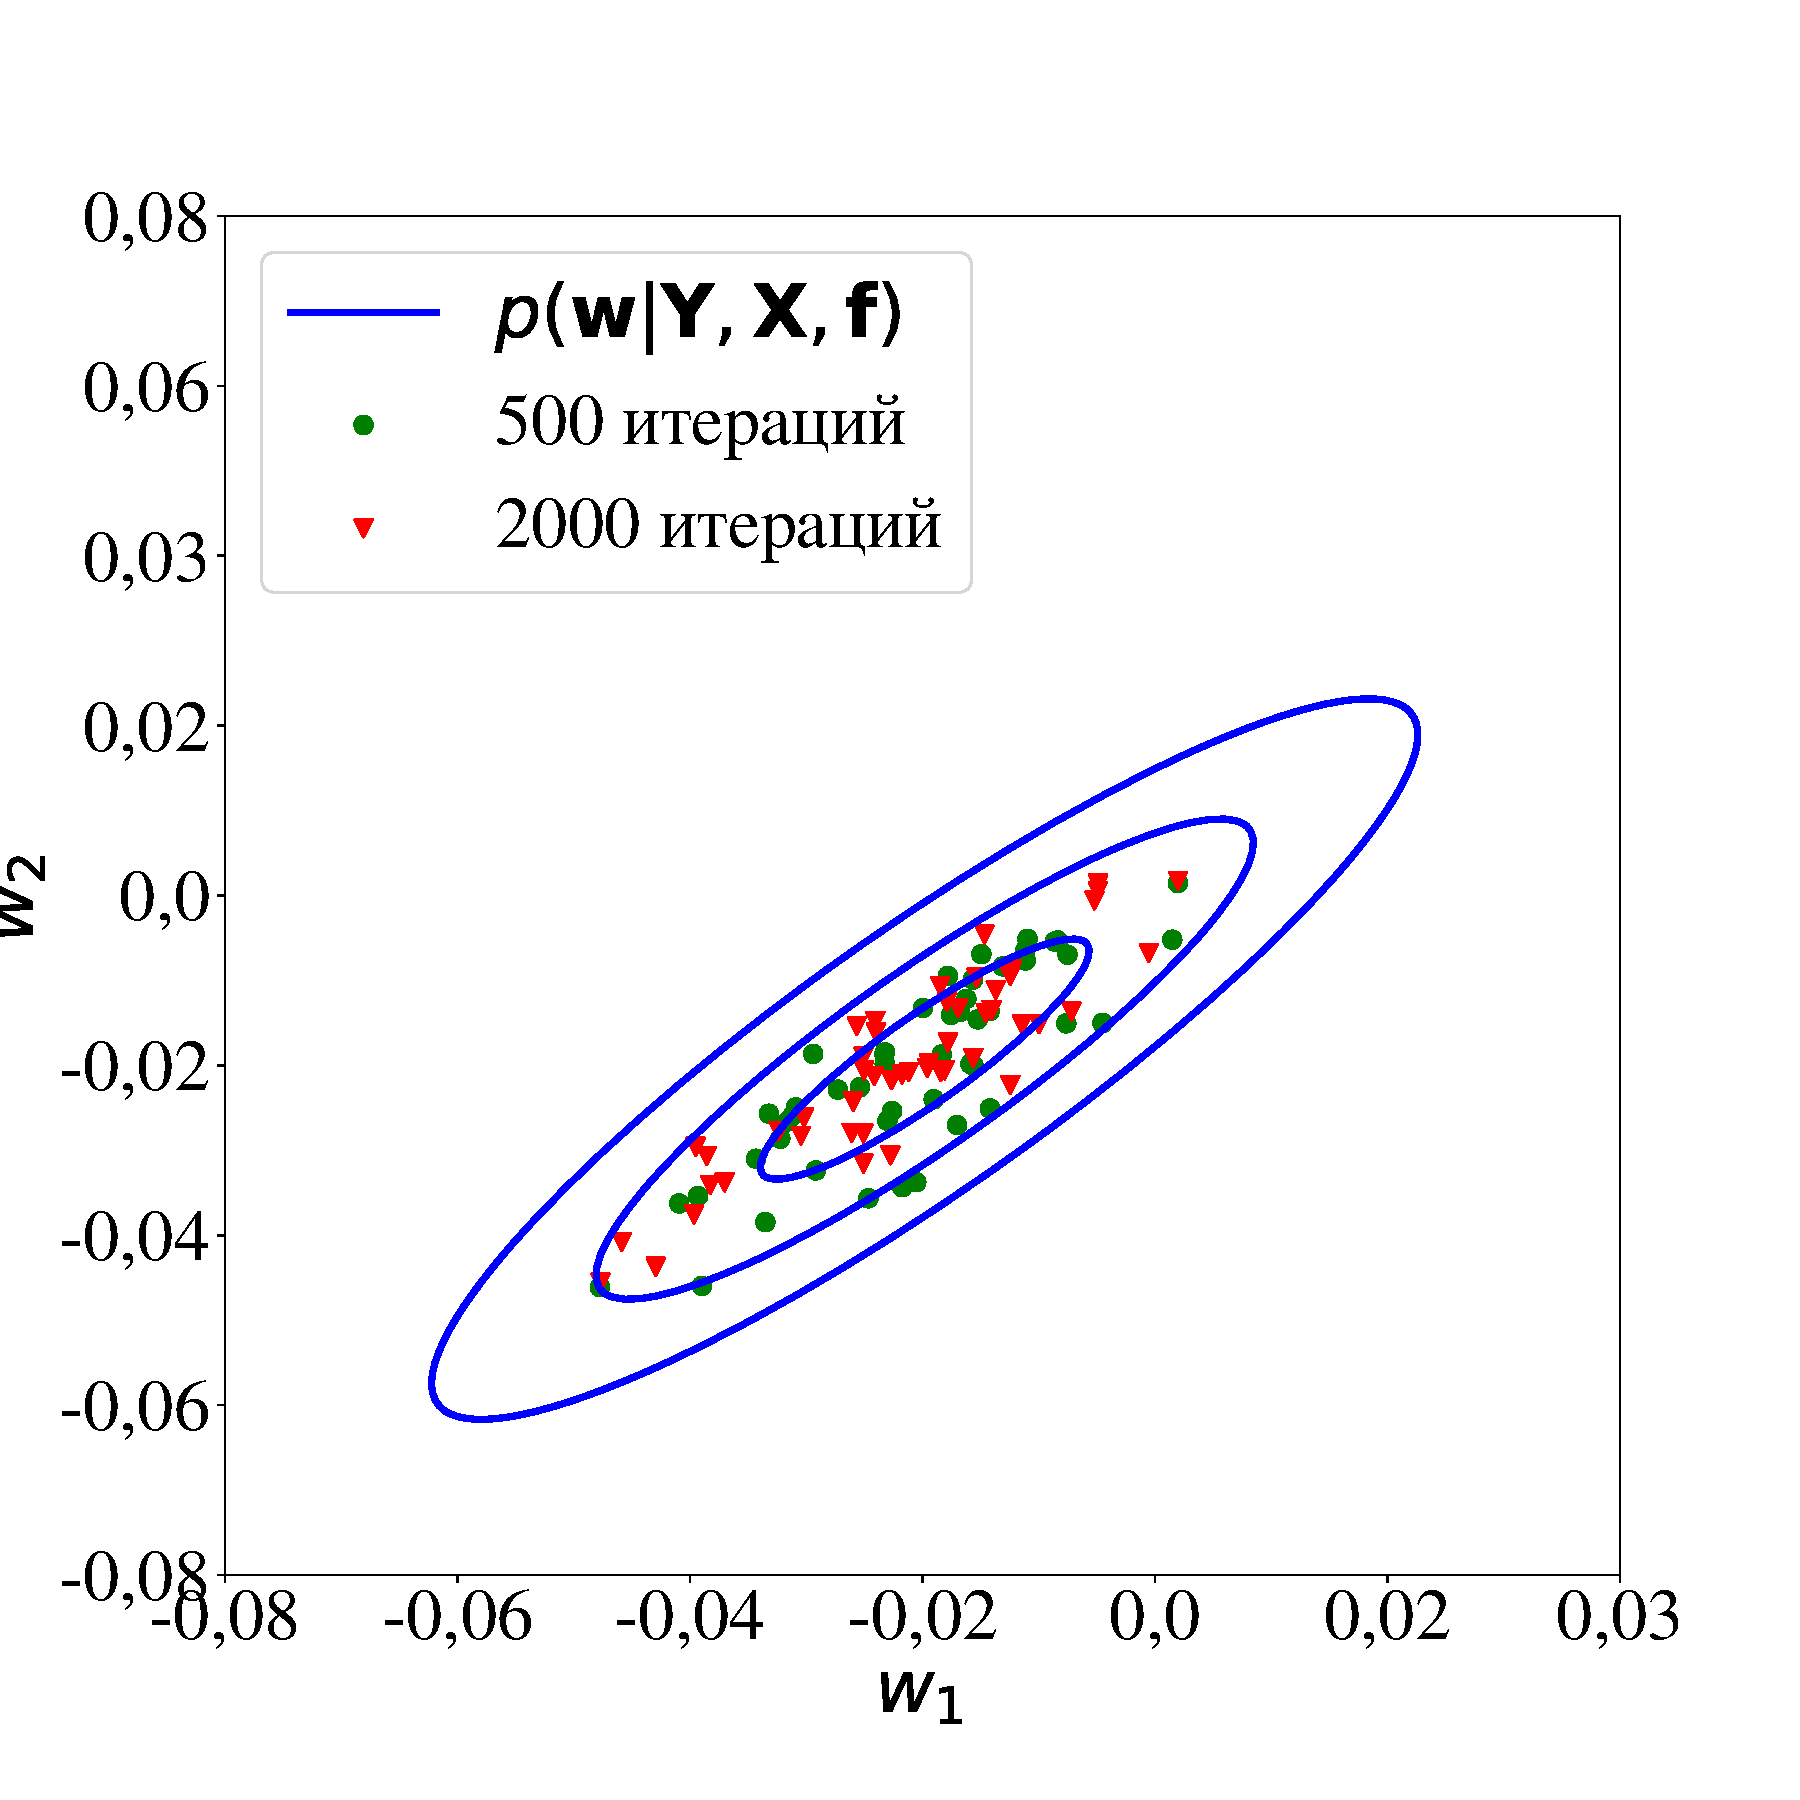
\includegraphics[width=\linewidth]{./plots/var/lang.pdf}
\endminipage\hfill
  \caption{Аппроксимация распределения \textit{а}) нормальным распределением, \textit{б}) распределением,
полученным с помощью градиентного спуска, \textit{в}) с использованием стохастической динамики Ланжевена.}
\label{fig:var}
\end{figure}




{Данный пример показывает, что качество итоговой аппроксимации распределения $p(\mathbf{w}|\mathbf{y}, \mathbf{X}, \mathbf{h})$ значительно зависит от схожести распределений $\hat{q}$ и $p(\mathbf{w}|\mathbf{y}, \mathbf{X}, \mathbf{h})$. В силу диагональности матрицы $\mathbf{A}_q$ и полного ранга матрицы $\mathbf{B}$  итоговое распределение $\hat{q}$ не может адекватно приблизить данное распределение  $p(\mathbf{w}|\mathbf{y}, \mathbf{X}, \mathbf{h})$.}

\end{example}

%\end{example_empty}
\textbf{Аппроксимация с использованием градиентного метода. }
В качестве множества распределений $\mathfrak{Q} = \{q(\mathbf{w})\}$, аппроксимирующих неизвестное распределение $\textnormal{log}~p(\mathbf{y}|\mathbf{X},\mathbf{h})$, используются распределения параметров, полученные в ходе их оптимизации. 

Представим неравенство~\eqref{eq:var_elbo}
\begin{equation}
\label{eq:var_elbo_entropy}
 \textnormal{log}~p(\mathbf{y}|\mathbf{X},\mathbf{h}) \geq \int_\mathbf{w} q(\mathbf{w})\textnormal{log}~\frac{p(\mathbf{y},\mathbf{w}|\mathbf{X}, \mathbf{h})}{q(\mathbf{w})}d\mathbf{w} =  \mathsf{E}_{q(\mathbf{w)}}\bigl(\textnormal{log~}p (\mathbf{y}, \mathbf{w}|\mathbf{X}, \mathbf{h})\bigr) - \mathsf{S}\bigl({q(\mathbf{w)}}\bigr),
\end{equation}
где $\mathsf{S}$ --- энтропия распределения:
\[
\mathsf{S}\bigl({q(\mathbf{w)}}\bigr) = - \int_{\mathbf{w}} q(\mathbf{w})\textnormal{log}~q(\mathbf{w})d\mathbf{w},
\]
$$p (\mathbf{y}, \mathbf{w}|\mathbf{X}, \mathbf{h}) = p (\mathbf{w}| \mathbf{h}) p (\mathbf{y}|\mathbf{X}, \mathbf{w}, \mathbf{h}),$$
$\mathsf{E}_{q(\mathbf{w)}}\bigl(\textnormal{log~}p (\mathbf{y}, \mathbf{w}|\mathbf{X}, \mathbf{h})\bigr)$ --- матожидание логарифма вероятности $\textnormal{log~}p (\mathbf{y}, \mathbf{w}|\mathbf{X}, \mathbf{h})$:
\[
	\mathsf{E}_{q(\mathbf{w)}}\bigl(\textnormal{log~}p (\mathbf{y}, \mathbf{w}|\mathbf{X}, \mathbf{h})\bigr) = \int_\mathbf{w} \textnormal{log~}p (\mathbf{y}, \mathbf{w}|\mathbf{X}, \mathbf{h}) q(\mathbf{w}) d\mathbf{w}.
\]

Оценка распределений производится при оптимизации параметров. Оптимизация выполняется в режиме мультистарта~\cite{multi}, т.е. при запуске оптимизации параметров модели из нескольких разных начальных приближений. Основная проблема такого подхода~---~вычисление энтропии $\mathsf{S}$ распределений $q(\mathbf{w}) \in Q$. Ниже представлен метод получения оценок энтропии~\eqref{eq:entropy} ~$\mathsf{S}$ и оценок правдоподобия~\eqref{eq:var_elbo_entropy}.

Запустим $r$ процедур оптимизаций модели $\mathbf{f}$ из разных начальных приближений:
\[
	L = -\sum_{l=1}^r \text{log}p(\mathbf{y}, \mathbf{w}^l|\mathbf{X}, \mathbf{h})  \to \min,
\] 
где $r$ --- число оптимизаций,
\begin{equation}
\label{eq:loss_func}
\text{log}p(\mathbf{y}, \mathbf{w}^l|\mathbf{X}, \mathbf{h}) = -\sum_{i=1}^m \textnormal{log}p({y}_i, \mathbf{w}^l |\mathbf{x}_i, \mathbf{h}) = -\textnormal{log}~p(\mathbf{w}^l|\mathbf{h}) - \sum_{i=1}^m \textnormal{log}p({y}_i |\mathbf{x}_i, \mathbf{w}^l, \mathbf{h}).
\end{equation}

Пусть начальные приближения параметров $\mathbf{w}^1, \dots, \mathbf{w}^r$ порождены из некоторого начального распределения $q^0(\mathbf{w})$:
\[ 
	\mathbf{w}^1, \dots, \mathbf{w}^r \sim q^0(\mathbf{w}). 
\]

Параметры $\mathbf{w}^1, \dots, \mathbf{w}^r$ задают вариационное распределение $q$: $$\boldsymbol{\theta} = [\mathbf{w}^1, \dots, \mathbf{w}^r].$$
%Обозначим за  $\mathbf{w}^l, g \in \{1,\dots,r\}$ значения параметров $\mathbf{w}^1, \dots, \mathbf{w}^r$ на  текущем шаге оптимизации. 


Для дальнейшего описания метода введем понятие оператора градиентного спуска, являющегося частным случаем оператора оптимизации~\eqref{eq:optim_operator}.
\begin{defin}
Оператором градиентного спуска назовем оператор оптимизации вида
\begin{equation}
\label{eq:sgd}
	T(\boldsymbol{\theta}) = \boldsymbol{\theta} - \beta \nabla L, 
\end{equation}
где  $\beta$ --- длина шага градиентного спуска.
\end{defin}

Пусть значения $\mathbf{w}^1, \dots, \mathbf{w}^r$  --- реализации случайной величины из некоторого распределения $q(\mathbf{w})$. Начальная энтропия распределения $q(\mathbf{w})$ соответствует энтропии распределения $q^0(\mathbf{w})$, из которого были порождены начальные приближения оптимизации параметров $\mathbf{w}^1, \dots, \mathbf{w}^r$. Под действием оператора $T$ распределение параметров $\mathbf{w}_1, \dots, \mathbf{w}_r$ изменяется. Для учета энтропии распределений, полученных в ходе оптимизации,
{ формализуем метод,  представленный в~\cite{early}. }

\begin{theorem}~Пусть $T$ --- оператор градиентного спуска,
 $L$ --- функция потерь, градиент $\nabla L$ которой имеет константу Липшица $C_L$.  Пусть $\mathbf{w}^1,\dots,\mathbf{w}^r$ ---  начальные приближения оптимизации модели, где $r$ --- число начальных приближений. Пусть $\beta$ --- длина шага градиентного спуска, такая что
\begin{equation}
\label{eq:ineq}
\beta<\frac{1}{C_L}, \quad \beta < \bigl(\max_{g \in \{1,\dots,r\}}\lambda_\textnormal{max} (\mathbf{H}(\mathbf{w}^l))\bigr)^{-1}, 
\end{equation}
где $\lambda_\textnormal{max}$ --- наибольшее по модулю собственное значение гессиана  $\mathbf{H}$ функции потерь $L$.

При выполнении неравенств~\eqref{eq:ineq} разность энтропий распределений $q'(\mathbf{w}), q(\mathbf{w})$ на смежных шагах почти наверное сходится к следующему выражению: 
\begin{equation}
\label{eq:entropy}
	\mathsf{S}\bigl(q'(\mathbf{w})) -  \mathsf{S}\bigl(q(\mathbf{w}))  \approx  \frac{1}{r}\sum_{l=1}^r \bigl(-\beta \textnormal{Tr}[\mathbf{H}(\mathbf{w}'^l)] - \beta \textnormal{Tr}[\mathbf{H}(\mathbf{w}'^l)\mathbf{H}(\mathbf{w}'^l)]  \bigr) + o_{\beta^2 \to 0}(1),
\end{equation}
где $\mathbf{H}$ --- гессиан функции потерь $L$.
\end{theorem}



\begin{proof}
Предварительно приведем две леммы, требуемые для доказательства теоремы.
\begin{lemma}[~\cite{sgd_conv}] Пусть $T$ --- оператор градиентного спуска, $L$ --- дважды дифференцируемая функция потерь, градиент $\nabla L$ которой имеет константу Липшица $C_L$.  Пусть для длины шага $\beta$ выполнено неравенство 
$
	\beta<\frac{1}{C_L}.
$
Тогда $T$ является диффеоморфизмом.
\end{lemma}

\begin{lemma}[~\cite{entropy}] Пусть $\mathbf{w}$ --- случайный вектор с непрерывным распределением $q(\mathbf{w})$. Пусть $T$ --- биективное отображение вектора $\mathbf{w}$ в пространство той же размерности. Пусть $q'(\mathbf{w})$ --- распределение вектора $T(\mathbf{w})$. Тогда справедливо утверждение
\begin{equation}
\label{eq:entropy_biject}
	\mathsf{S}\bigl(q'(\mathbf{w})\bigr) -  \mathsf{S}\bigl(q(\mathbf{w})\bigr)  = \int_\mathbf{w}  q'(\mathbf{w}) \textnormal{log}~\left|\frac{\partial{T(\mathbf{w})}}{\partial{\mathbf{w}}}\right| d\mathbf{w}.
\end{equation}
\end{lemma}



Рассмотрим очередной шаг оптимизации. При $\beta<\frac{1}{C}$ оператор градиентного спуска $T$ является диффеоморфизмом, а значит, и биекцией, справедлива формула~\eqref{eq:entropy_biject}.
По усиленному закону больших чисел 
\[
	\mathsf{S}\bigl(q'(\mathbf{w})\bigr) -  \mathsf{S}\bigl(q(\mathbf{w})\bigr)  \approx  \frac{1}{r}\sum_{l=1}^r \textnormal{log}~\left|\frac{\partial{T(\mathbf{w}'^l)}}{\partial{\mathbf{w}}}\right|.
\]
Логарифм якобиана  $\textnormal{log}~\left|\frac{\partial{T(\mathbf{w}'^l)}}{\partial{\mathbf{w}}}\right|$ оператора $T$ запишем как%~\cite{early}:
\begin{equation}
\label{eq:to_taylor}
	\textnormal{log}~\left|\frac{\partial{T(\mathbf{w}'^l)}}{\partial{\mathbf{w}}}\right| = \textnormal{log}~|\mathbf{I} - \beta\mathbf{H}| = \sum_{i=1}^{u} \textnormal{log}~(1-\beta\lambda_i),
\end{equation}
где $\lambda_i$ --- $i$-е собственное значение гессиана $\mathbf{H}$.

При $(\beta\lambda_i) ^ 2 \leq (\beta\lambda_\textnormal{max})^2 < 1$ выражение~\eqref{eq:to_taylor} раскладывается в ряд Тейлора:
\[
	 \sum_{t=1}^{u} \textnormal{log}~(1-\beta\lambda_i) =  -\beta \textnormal{Tr}[\mathbf{H}(\mathbf{w}'^l)] - \beta^2 \textnormal{Tr}[\mathbf{H}(\mathbf{w}'^l)\mathbf{H}(\mathbf{w}'^l)] + o_{\beta^2 \to 0}(1).
\]
Просуммировав полученные выражения для каждой точки мультистарта и вынеся $o_{\beta^2 \to 0}(1)$ за скобки, получим выражение~\eqref{eq:entropy}, что и требовалось доказать.

\end{proof} 	


Получим итоговую формулу для оценки правдоподобия модели.
\begin{theorem}\label{st:st2}
Оценка~\eqref{eq:var_elbo_entropy} на шаге оптимизации $\tau$ представима в виде
\begin{equation}
\label{eq:ev_grad_full}
\textnormal{log}~\hat{p}(\mathbf{y}|\mathbf{X}, \mathbf{h}) \approx \frac{1}{r} \sum_{g = 1}^r L(\mathbf{w}^l_\tau, \mathbf{X}, \mathbf{y})  + 
\end{equation}
\[
+\mathsf{S}\big(q^0(\mathbf{w})\bigr) + \frac{1}{r}\sum_{b=1}^\tau\sum_{l=1}^r \bigl(-\beta \textnormal{Tr}[\mathbf{H}(\mathbf{w}_b^l)] - \beta^2 \textnormal{Tr}[\mathbf{H}(\mathbf{w}_b^l)\mathbf{H}(\mathbf{w}_b^l)]  \bigr) 
\]
с точностью до слагаемых вида $o_{\beta^2 \to 0}(1)$,
где $\mathbf{w}_b^l$ --- $l$-я реализация параметров модели на шаге оптимизации $b$, $q^0(\mathbf{w})$ --- начальное распределение.
\end{theorem}



\begin{proof} Представим энтропию распределения $q^\tau(\mathbf{w})$ следующим образом:
\[
\mathsf{S}\bigl(q^\tau(\mathbf{w})\bigr) = \mathsf{S}\bigl(q^0(\mathbf{w})\bigr) - \mathsf{S}\bigl(q^0(\mathbf{w})\bigr) + \mathsf{S}\bigl(q^1(\mathbf{w})\bigr) - \mathsf{S}\bigl(q^1(\mathbf{w})\bigr) +\dots -
\mathsf{S}\bigl(q^{\tau-1}(\mathbf{w})\bigr) + \mathsf{S}\bigl(q^\tau(\mathbf{w})\bigr).
\]
Каждая разность энтропий вида $\mathsf{S}\bigl(q^b(\mathbf{w})\bigr) - \mathsf{S}\bigl(q^{b-1}(\mathbf{w})\bigr)$ по теореме с точностью до $o_{\beta^2 \to 0}(1)$ представима в виде
\begin{equation}
\label{eq:eq_sums}
	\mathsf{S}\bigl(q^b(\mathbf{w})\bigr) -  \mathsf{S}\bigl(q^{b-1}(\mathbf{w})\bigr)  \approx  \frac{1}{r}\sum_{l=1}^r \bigl(-\beta \textnormal{Tr}[\mathbf{H}(\mathbf{w}_b^l)] - \beta^2 \textnormal{Tr}[\mathbf{H}(\mathbf{w}_b^l)\mathbf{H}(\mathbf{w}_b^l)]  \bigr).
\end{equation}

Формула~\eqref{eq:ev_grad_full} получается подстановкой в выражение~\eqref{eq:var_elbo_entropy} суммы выражений вида~\eqref{eq:eq_sums}, а также начальной энтропии $\mathsf{S}\bigl(q^0(\mathbf{w}))$.
\end{proof}

В~\cite{early} предлагается алгоритм приближенного вычисления для выражения, находящегося под знаком суммы в~\eqref{eq:ev_grad_full}:
\[
	-\beta \textnormal{Tr}[\mathbf{H}(\mathbf{w}^l)] - \beta^2 \textnormal{Tr}[\mathbf{H}(\mathbf{w}^l)\mathbf{H}(\mathbf{w}^l)]  \approx \mathbf{r}_0^\mathsf{T}\bigl(-2\mathbf{r}_0 + 3\mathbf{r}_1 -\mathbf{r}_2\bigr),
\]
где вектор $\mathbf{r}_0$  порождается из нормального распределения:
$$\mathbf{r}_0 \sim \mathcal{N}(\mathbf{0}, \mathbf{I}), \quad \mathbf{r}_1 = \mathbf{r}_0 - \beta \mathbf{r}_0^\mathsf{T} \nabla \nabla L, \quad \mathbf{r}_2 = \mathbf{r}_1 - \beta \mathbf{r}_1^\mathsf{T} \nabla \nabla L.$$


Заметим, что при приближении параметров модели к точке экстремума оценка правдоподобия устремляется в минус бесконечность в силу постоянно убывающей энтропии. Таким образом, чем ближе градиентный метод приближает параметры модели к точке экстремума, тем менее точной становится оценка правдоподобия модели. Один из методов борьбы с данной проблемой представлен в следующих параграфах.
\begin{figure}
\caption{Псевдокод алгоритма получения вариационной нижней оценки правдоподобия модели с использованием градиентного спуска}
\label{fig:algo}
\begin{algorithmic}[1]
\REQUIRE $\mathbf{X}, \mathbf{y}, p(\mathbf{w}|\mathbf{h})$;
\REQUIRE критерий останова $\text{Stop}$, начальное распределение параметров $q^0$, количество точек мультистарта $r$, функция потерь $L$, ее первая и вторая производные;
\ENSURE $\textnormal{log}~\hat{p}(\mathbf{y}|\mathbf{X}, \mathbf{h})$;
\FOR{$l=1,\dots,r$}
\STATE $\mathbf{w}^l \sim q^0$;
\ENDFOR
\STATE $\mathsf{S} = \mathsf{S}\bigl(q^0)$;
\WHILE{не достигнут критерий останова $\text{Stop}$}
\STATE $\boldsymbol{\theta} = T(\boldsymbol{\theta});$
\FOR{$l=1,\dots,r$}
\STATE $\mathbf{r}_0 \sim \mathcal{N}(\mathbf{0}, \mathbf{I})$;
\STATE $\mathbf{r}_1 = \mathbf{r}_0 - \beta \mathbf{r}^{\mathsf{T}}_0 \nabla \nabla L(\mathbf{w}^l, \mathbf{y}, \mathbf{X})$;
\STATE $\mathbf{r}_2 = \mathbf{r}_1 - \beta \mathbf{r}^{\mathsf{T}}_1 \nabla \nabla L(\mathbf{w}^l, \mathbf{y}, \mathbf{X})$;
\STATE $\mathsf{S}^l = \mathbf{r}_0^\mathsf{T}\bigl(-2\mathbf{r}_0 + 3\mathbf{r}_1 -\mathbf{r}_2\bigr)$;
\ENDFOR
\STATE $\mathsf{S} = \frac{1}{r}\sum_{l=1}^r \mathsf{S}^l$;
\ENDWHILE
\STATE $\hat{p}(\mathbf{y}|\mathbf{X}, \mathbf{w}, \mathbf{h}) = \frac{1}{r}\sum_{l=1}^r p(\mathbf{y}|\mathbf{X}, \mathbf{w}^l, \mathbf{h})$;
\STATE $\hat{p}(\mathbf{w} | \mathbf{h}) = \frac{1}{r}\sum_{l=1}^r p(\mathbf{w}^l| \mathbf{h})$;
\STATE $\textnormal{log}~\hat{p}(\mathbf{y}|\mathbf{X}, \mathbf{h}) = \textnormal{log}~\hat{p}(\mathbf{y}|\mathbf{X}, \mathbf{w}, \mathbf{h}) +\textnormal{log}~\hat{p}(\mathbf{w} | \mathbf{h})$;
	
\end{algorithmic}
\end{figure}



\textbf{Модификация алгоритма оптимизации модели.} \\
В качестве оператора $T$ предлагается использовать псевдослучайный стохастический градиентный спуск, т.е. градиентный спуск~\eqref{eq:sgd_operator}, оптимизирующий параметры $\mathbf{w}^1,\dots,\mathbf{w}^r$ по некоторой случайной подвыборке $\hat{\mathbf{X}}, \hat{\mathbf{y}}$, одинаковой для каждой точки старта $\mathbf{w}^1,\dots,\mathbf{w}^r$:
\[
    T( \boldsymbol{\theta}| L,\mathbf{X},  \mathbf{y},  \mathbf{h}, \boldsymbol{\beta}) = \boldsymbol{\theta} - \beta\nabla L(\boldsymbol{\theta},   \mathbf{h},  \hat{\mathbf{X}}, \hat{\mathbf{y}}),
\]
где $\beta_{\text{lr}}$ --- шаг градиентного спуска, $\hat{\mathbf{y}}, \hat{\mathbf{X}}$ --- случайная подвыборка заданной мощности выборки $\mathfrak{D}$.

где $\hat{\mathbf{X}}$ --- случайная подвыборка выборки ${\mathbf{X}}$, одинаковая для всех точек мультистарта, $\hat{\mathbf{y}}$ --- соответствующие метки классов, $$|\hat{\mathbf{X}}| = \hat{m}.$$

Как и версия алгоритма с использованием градиентного спуска~\eqref{eq:sgd}, основной проблемой модифицированного алгоритма оценки интеграла~\eqref{eq:var_elbo2} является грубость аппроксимации исходного распределения $p(\mathbf{w}|\mathbf{f},\mathfrak{D})$.

Рассмотрим пример~\eqref{eq:example_post}.
График аппроксимации распределения $p(\mathbf{w}|\mathbf{y}, \mathbf{X}, \mathbf{h})$ представлен на рис.~\ref{fig:var},\textit{б}.
Как видно из графика, градиентный спуск сходится к моде распределения. При небольшом количестве итераций полученное распределение также слабо аппроксимирует апостериорное распределение. {При приближении к точке экстремума снижается вариационная оценка правдоподобия модели, что  интерпретируется как возможное начало переобучения~\cite{early}. Таким образом, снижение оценки~\eqref{eq:ev_grad_full} можно использовать как критерий остановки оптимизации модели для снижения эффекта переобучения.  }

На рис.~\ref{fig:var} представлена  {аппроксимация распределения $p(\mathbf{w}|\mathbf{Y}, \mathbf{X}, \mathbf{h})$ различными методами: \textit{а}) нормальным распределением с диагональной матрицей ковариаций, \textit{б}) с помощью градиентного спуска, \textit{в}) с помощью стохастической динамики Ланжевена. Точками отмечены параметры модели $\mathbf{f}$, полученные в ходе нескольких запусков оптимизации и являющиеся реализациями случайной величины с распределением $q(\mathbf{w})$. Нормальное распределение слабо аппроксимирует распределение $p(\mathbf{w}|\mathbf{Y}, \mathbf{X}, \mathbf{h})$ в силу диагональности матрицы ковариаций. Распределение, полученное с помощью градиентного спуска, слабо аппроксимирует распределение $p(\mathbf{w}|\mathbf{Y}, \mathbf{X}, \mathbf{h})$, так как сходится к моде.}





\textbf{Аппроксимация с использованием динамики Ланжевена}\\
Для достижения нижней оценки интеграла~\eqref{eq:var_elbo2}, более близкой к реальному значению логарифма интеграла~\eqref{eq:evidence}, чем оценка с использованием градиентного спуска, предлагается использовать стохастическую динамику Ланжевена~\cite{langevin}. Стохастическая динамика Ланжевена представляет собой вариант стохастического градиентного спуска с добавлением гауссового шума:
\begin{equation}
\label{eq:langevin}
	T(\mathbf{w}) = \mathbf{w} -  \beta \nabla L -\frac{m}{\hat{m}}\textnormal{log}p(\hat{\mathbf{y}}|\hat{\mathbf{X}}, \mathbf{w},\mathbf{h}) + \boldsymbol{\varepsilon}, \quad  \boldsymbol{\varepsilon} \sim \mathcal{N}(\mathbf{0}, {\frac{\beta}{2}}\mathbf{I}),
\end{equation}
где $\hat{\mathbf{X}}$ --- псевдослучайная подвыборка, $\hat{\mathbf{y}}$ --- соответствующие метки, $\hat{m}$ --- размер подвыборки. Длина шага оптимизации $\beta$ удовлетворяет  {условиям, гарантирующим сходимость алгоритма в стандартных ситуациях~\cite{langevin}}:
\[
	\sum_{\tau=1}^\infty \beta_\tau = \infty, \quad \sum_{\tau=1}^\infty \beta_\tau^2 < \infty.
\]

Для оценки энтропии с учетом шума $\boldsymbol{\varepsilon}$ предлагается использовать следующее неравенство~\cite{entropy,var_grad}:
\[
\hat{\mathsf{S}}\bigl(q^\tau(\mathbf{w})\bigr)   \geq \frac{1}{2}u\textnormal{log}\left(\textnormal{exp}\left(\frac{2\mathsf{S}\bigl(q^\tau(\mathbf{w})\bigr)}{u}\right) + \textnormal{exp}\left(\frac{2\mathsf{S}\bigl( \boldsymbol{\varepsilon})}{u}\right)\right),
\]
{где  $\tau$ --- текущий шаг оптимизации,} $\mathsf{S}\bigl( \mathcal{N}({0}, {\frac{\beta}{2}})\bigr)$ --- энтропия нормального распределения, $\hat{\mathsf{S}}(q^\tau(\mathbf{w}))$ --- энтропия распределения $q^\tau$ с учетом добавленного шума~$\boldsymbol{\varepsilon}$.


В отличие от стохастического градиентного спуска стохастическая динамика Ланжевена сходится к апостериорному распределению параметров $p(\mathbf{w}|\mathfrak{D},\mathbf{h})$~\cite{langevin, langevin_sato}.  График аппроксимации апостериорного распределения с использованием динамики Ланжевена представлен на рис.~\ref{fig:var},\textit{в}. При одинаковом количестве итераций динамика Ланжевена продолжает аппроксимировать апостериорное распределение, в то время как градиентный спуск сходится к моде распределения. {Как видно из графика, алгоритм, основанный на стохастической динамике Ланжевена, способен давать более точную вариационную оценку правдоподобия~\eqref{eq:var_elbo2}. В то же время алгоритм более требователен к настройке параметров оптимизации~\cite{sgld}: \textit{``быстро изменяющаяся кривизна [траекторий параметров модели] делает методы стохастической градиентной динамики Ланжевена по умолчанию неэффективными''.}}
%However, the rapidly changing curvature renders default SGLD methods inefficient




\section{Анализ методов выбора моделей}
Для анализа свойств предложенного критерия субоптимальности в задачах регрессии и классификации, а также методов получения нижних оценок правдоподобия модели в задачах выбора моделей был проведен ряд вычислительных экспериментов на выборках Boston Housing, Protein Structure, а также на небольшой подвыборке YearPredictionMSD (далее --- Boston, Protein и MSD)~\cite{UCI} {и подвыборке изображений рукописных цифр MNIST~\cite{mnist}}.

{Для выборок Boston, Protein и MSD} была рассмотрена задача регрессии
\[
	\mathbf{y} = \mathbf{f}(\mathbf{X}, \mathbf{w}) + \boldsymbol{\varepsilon}, \quad  \boldsymbol{\varepsilon} \sim \mathcal{N}(\mathbf{0}, \mathbf{I}), \mathbf{f} \in {M}.
\]

В качестве множества моделей $M$ были рассмотрены  нейросети с одним скрытым слоем и softplus-функцией активации:
\begin{equation}
\label{eq:model}
	\mathbf{f}(\mathbf{w}, \mathbf{X}) =   \textbf{softplus}\bigl(\mathbf{X} \mathbf{W}_1 \bigr)  \mathbf{W}_2,
\end{equation}
где $\mathbf{W}_1 \in \mathbb{R}^{n\times n_1}$ --- матрица параметров скрытого слоя нейросети, $\mathbf{W}_2 \in \mathbb{R}^{n_1\times 1}$ --- матрица параметров выходного слоя нейросети, {$\textbf{softplus}(\mathbf{X}) = \textbf{log}\bigl(1+\textbf{exp}(\mathbf{X})\bigr)$}.

{Для выборки Boston также было рассмотрено множество моделей с тремя скрытыми слоями, построенных аналогично однослойной модели~\eqref{eq:model}. Размер каждого слоя равнялся 50.}

{Для выборки MNIST была рассмотрена задача бинарной классификации: из выборки были взяты только объекты, соответствующие цифрам 7 и 9. Размерность выборки была понижена с 784 до 50 методом главных компонент аналогично~\cite{firefly}. Для анализа моделей, полученных в случае высокой вероятности переобучения, из обучающей выборки были взяты первые 500 объектов. В качестве модели рассматривалась нейросеть с тремя скрытыми слоями}
\[
    \mathbf{f}(\mathbf{w}, \mathbf{X}) =   \boldsymbol{\sigma}(\textbf{softplus}\bigl(  \textbf{softplus} \bigl(\textbf{softplus}\bigl(\mathbf{X} \mathbf{W}_1 \bigr)  \mathbf{W}_2 \bigr) \mathbf{W}_3 \bigr) \mathbf{W}_4),
\]
{где $\boldsymbol{\sigma}(\mathbf{X}) = \bigl(1+\textbf{exp}(\mathbf{-X})\bigr)^{-1}$  --- сигмоида, $\mathbf{W}_1, \dots, \mathbf{W}_4$ --- параметры нейросети.}



Во всех экспериментах исходная выборка $\mathfrak{D}$ разбивалась на обучающую и контрольную подвыборки:
$
	\mathfrak{D} = \mathfrak{D}_\textnormal{train} \sqcup \mathfrak{D}_\textnormal{text}.
$

Оптимизация параметров производилась на подвыборке $\mathfrak{D}_\textnormal{train}$. Для контроля переобучения некоторых алгоритмов из обучающей выборки $\mathfrak{D}_\textnormal{train}$ формировалась валидационная выборка $\mathfrak{D}_\textnormal{valid}$, на которой не проводилась оптимизация параметров  модели. Мощность валидационной выборки $\mathfrak{D}_\textnormal{valid}$ составляла 0,1 мощности обучающей выборки  $\mathfrak{D}_\textnormal{train}$, объекты для валидационной выборки выбирались случайным образом независимо для каждого старта алгоритма.
Качество полученных моделей проверялось на подвыборке $\mathfrak{D}_\textnormal{test}.$ Критерием качества модели выступали среднеквадратичное отклонение вектора $\mathbf{y}$ от вектора $\mathbf{f}(\mathbf{w}, \mathbf{X})$ (RMSE) {в случае задачи регрессии и доля верно предсказанных меток класса (Accuracy) в задаче классификации}, а также { соответствующие критерии } при возмущении элементов выборки:
\begin{equation}
\label{eq:rmse}
	\textnormal{RMSE}_{\sigma} =\textnormal{RMSE}\bigl(\mathbf{f}( \mathbf{w}, \mathbf{X}+\boldsymbol{\varepsilon}), \mathbf{y}\bigr),  \quad \boldsymbol{\varepsilon} \sim \mathcal{N}(\mathbf{0}, \sigma \mathbf{I}).
\end{equation}

Были рассмотрены шесть алгоритмов.
\begin{enumerate}
\item Базовый алгоритм: оптимизация параметров без валидации и ранней остановки. Оптимизация проводилась с использованием стохастического градиентного спуска~\eqref{eq:sgd}. Для данного алгоритма априорное распределение $p(\mathbf{w}|\mathbf{h})$ не использовалось.
\item Алгоритм с валидацией. Для контроля переобучения во время оптимизации качество модели оценивалось на валидационной выборке $\mathfrak{D}_\textnormal{valid}$. Для данного алгоритма априорное распределение также не использовалось.
\item Алгоритм с валидацией и введенным априорным распределением. В качестве априорного распределения рассматривается распределение вида
$
	\mathbf{w} \sim \mathcal{N}(\mathbf{0}, \alpha \mathbf{I}), 
$
где $\alpha$ --- дисперсия.

\item Нахождение вариационной нижней оценки с использованием стохастического градиентного спуска.
\item Нахождение вариационной нижней оценки с использованием стохастической динамики Ланжевена.
\item Нахождение вариационной нижней оценки с аппроксимацией нормальным распределением ~\eqref{eq:gaus}.
\end{enumerate}




Параметры модели выбирались из точек мультистарта (алгоритмы 1---5) или порождались из распределения $\hat{q}$ (алгоритм 6). Количество точек мультистарта: $r=10$ {для задач регрессии и $r=25$ для задачи классификации}.
Для алгоритмов 2---6 применялась ранняя остановка: каждые $\tau_\textnormal{val}$ итераций производилась оценка внутреннего критерия качества модели. В качестве критерия остановки применялось следующее условие: значение внутреннего критерия качества не улучшалось $3\tau_\textnormal{val}$ итераций. Для разных алгоритмов внутренним критерием качества выступали различные величины:
\begin{enumerate}
\item функция потерь $L$~\eqref{eq:loss_func} на валидационной выборке $\mathfrak{D}_\textnormal{valid}$ для алгоритмов $2,3$,
\item вариационная нижняя оценка правдоподобия~\eqref{eq:var_elbo} на обучающей выборке $\mathfrak{D}_\textnormal{train}$ для алгоритмов $4,5,6$.
\end{enumerate}

Для каждой модели назначались различные значения параметра $\alpha (\alpha \in \{10, \dots, 10^9\})$ и длины шага оптимизации $\beta$, отбирались наилучшие модели. 



Описание эксперимента представлено в табл.~1. Результаты экспериментов представлены в табл.~2. На рис.~\ref{fig:noise_in_data} представлен график зависимости $\textnormal{RMSE}_{\sigma}$ от параметра~$\sigma$~{ для однослойных моделей}. 

\begin{figure}[tbh!]


\minipage{0.32\textwidth}
\caption*{\textit{а}}
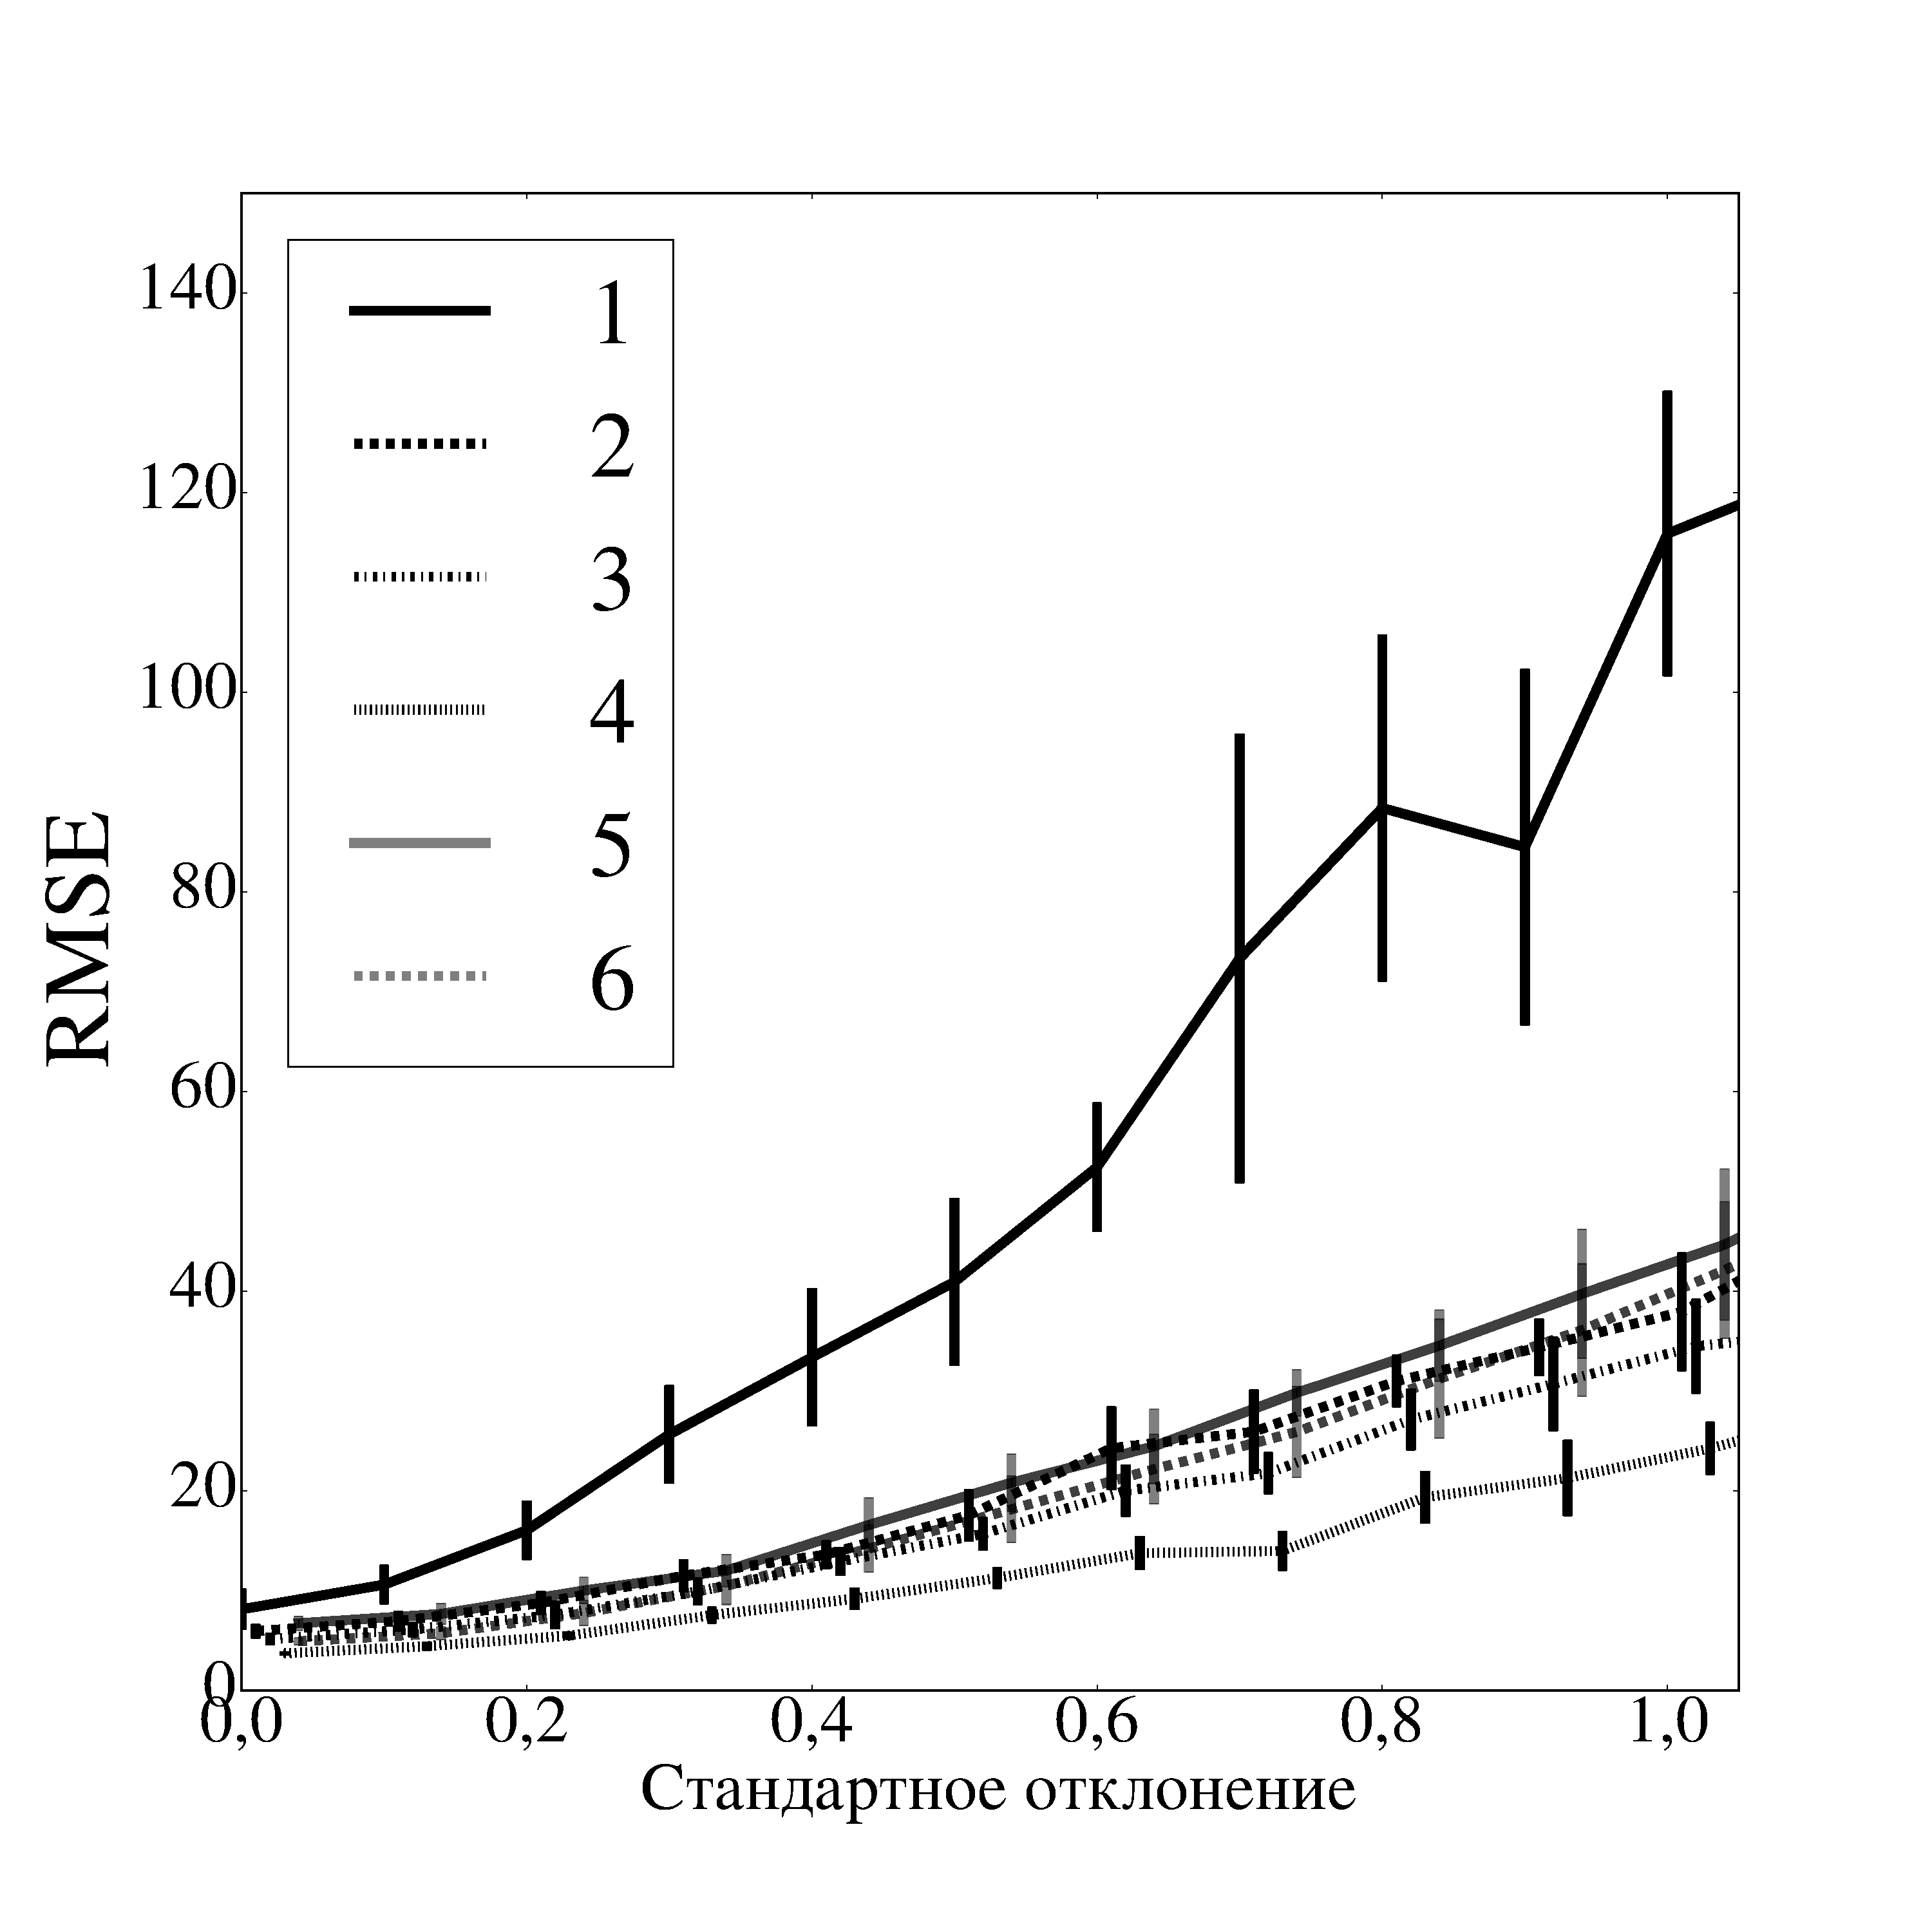
\includegraphics[width=1.0\textwidth]{./plots/var/boston/rmse_data2.pdf}
\endminipage\hfill
\minipage{0.32\textwidth}
\caption*{\textit{б}}
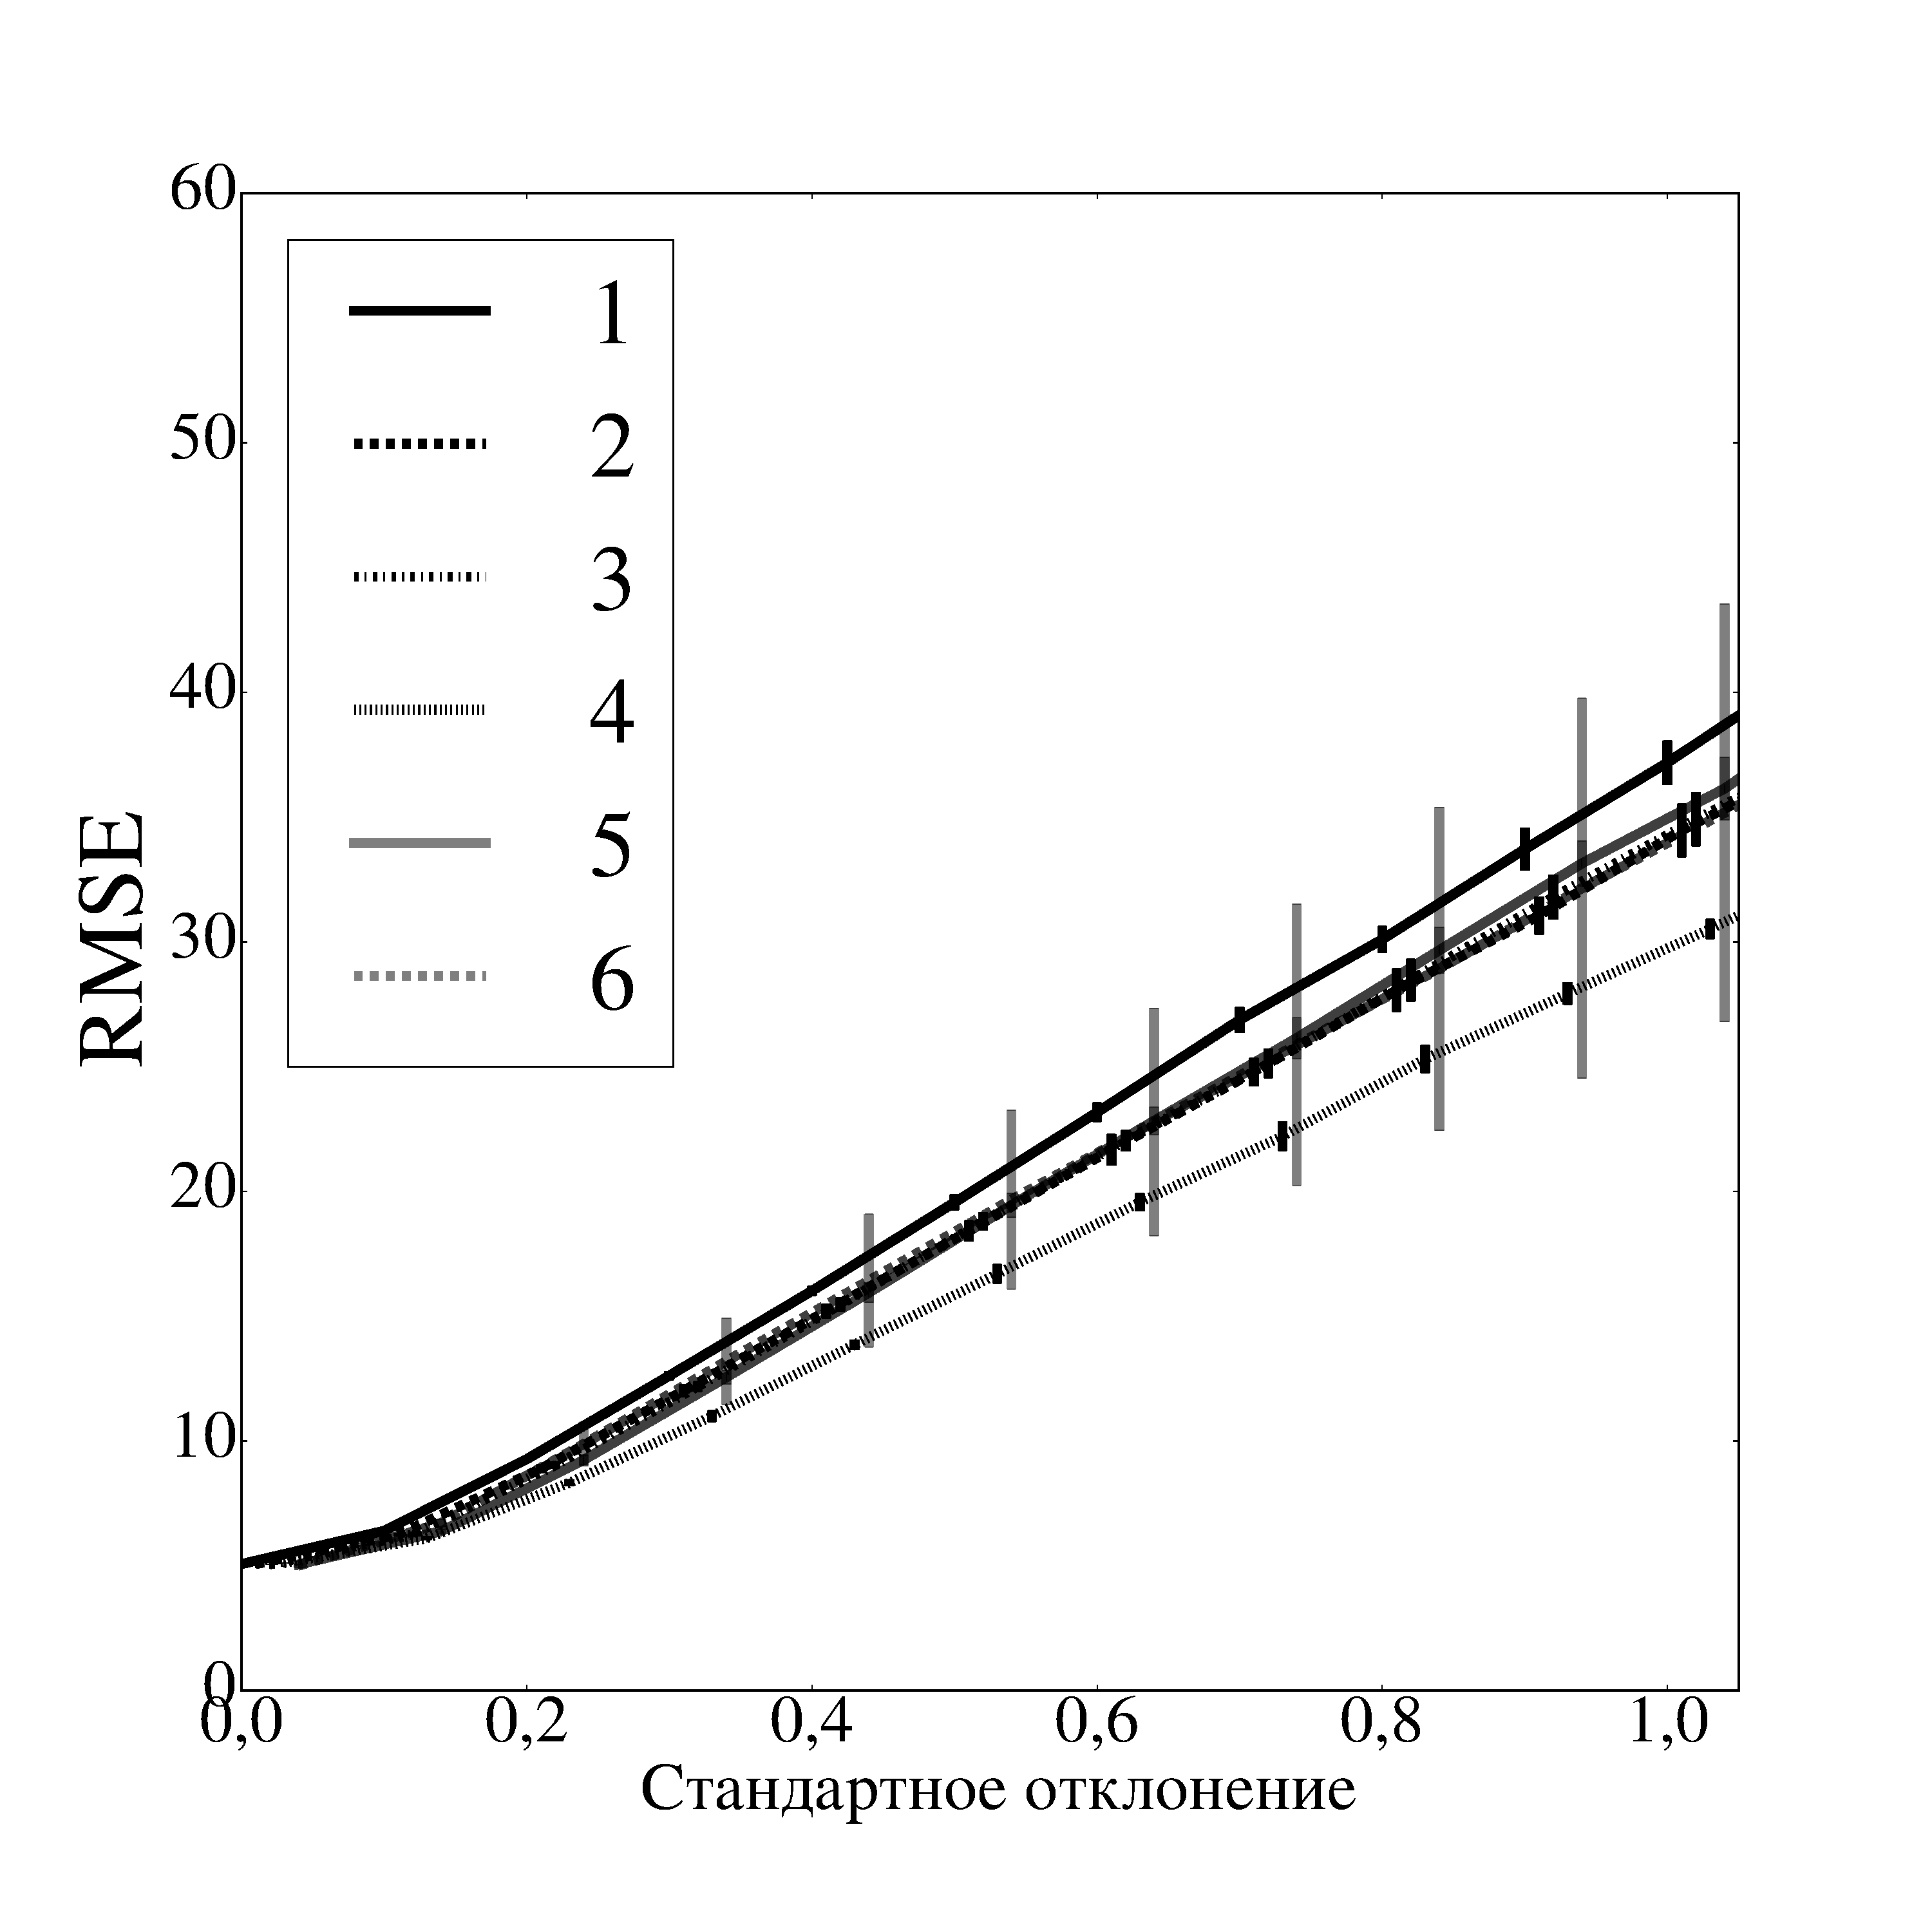
\includegraphics[width=1.0\textwidth]{./plots/var/protein/rmse_data2.pdf}

\endminipage\hfill
\minipage{0.32\textwidth}%
\caption*{\textit{в}}
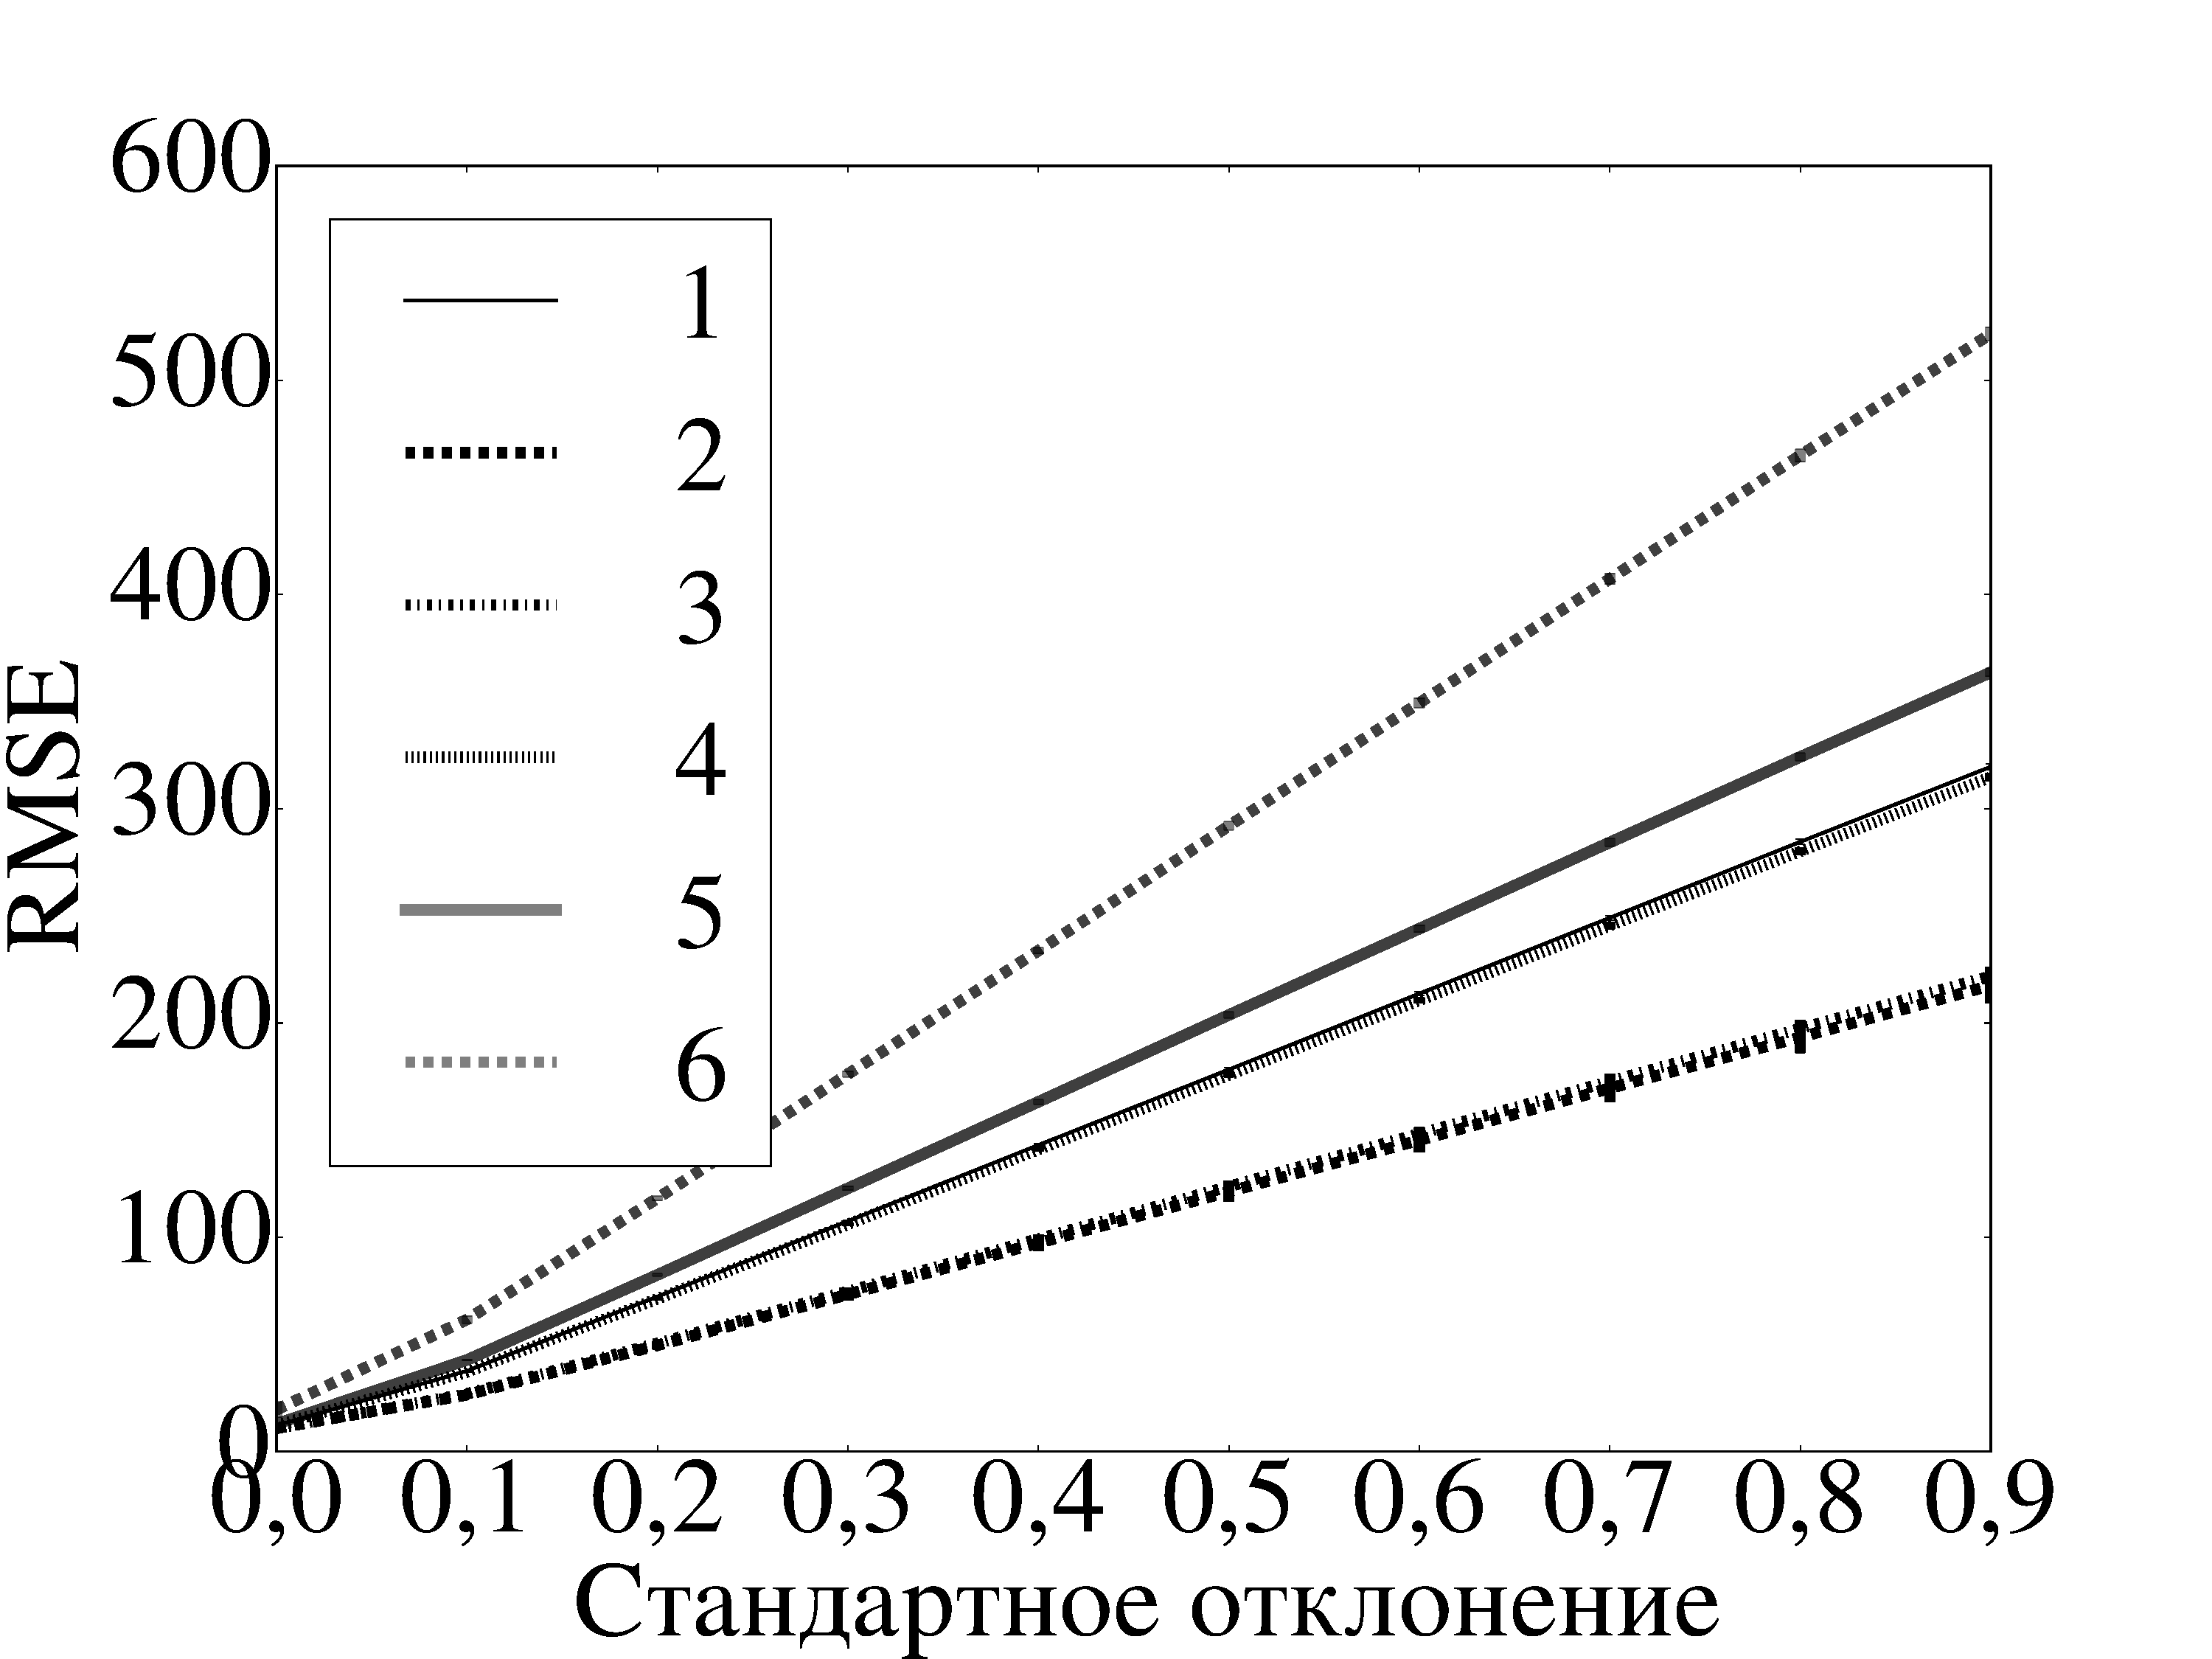
\includegraphics[width=1.0\textwidth]{./plots/var/msd/rmse_data2.pdf}

\endminipage
\caption{ Возмущение выборки для однослойных нейросетей: \textit{а}) Boston Housing, \textit{б}) Protein, \textit{в}) MSD.
}
\label{fig:noise_in_data}
\end{figure}




\begin{table}[!htbp]
\captionsetup{justification=raggedright,singlelinecheck=false}
\label{table1}
\caption{Описание выборок для экспериментов  по выбору моделей}
\footnotesize
\centering

\begin{tabular}{ | p{2cm} |p{2cm} | p{2cm} | p{2cm} | p{2cm} | p{2cm} | }
\hline
Выборка $\mathfrak{D}$ & Интервал валидации, $\tau_\textnormal{val}$ & Количество объектов, $m$ & Количество признаков, $n$ & Размер подвыборки, $\hat{m}$ &  Размер скрытого слоя, $n_1$ \\
\hline
Boston Housing & 100 & 506 & 13 & $\hat{m} = m$ & 50 \\
\hline
Protein & 1000 & 45000 & 9 & $\hat{m} = 200$ & 100 \\
\hline
MSD & 1000& 5000 & 91 & $\hat{m} = 50$ & 100\\
\hline
MNIST & 100  & 500 & 50 & $\hat{m} = 100$ & 50\\ 
\hline
\end{tabular}
\end{table}


\newcommand{\specialcell}[2][c]{%
  \begin{tabular}[#1]{@{}c@{}}#2\end{tabular}}

\begin{table}[htbp!]
\captionsetup{justification=raggedright,singlelinecheck=false}
\centering
\label{table2}
\caption{Результаты эксперимента по выбору моделей}
\footnotesize
\begin{tabular}{ | c | c | c | c | c | c | c |}

\hline
&\multicolumn{6}{|c|}{Алгоритмы}  \\
\hline
Выборка $\mathfrak{D}$ & 1 & 2 & 3 & 4 & 5 & 6 \\
\hline
\multicolumn{7}{|c|}{Результаты, RMSE/Accuracy}  \\

\hline
\specialcell{ Boston,  \\один  слой} & 8,1  $\pm$ 2,0 & 5,9 $\pm$ 0,7 & 5,2 $\pm$ 0,6 & $\mathbf{3,7 \pm 0,2}$ & 6,7 $\pm$ 0,7 & 5,0 $\pm$ 0,4 \\
\hline
Boston, 3 слоя & 7,1 $\pm$ 1,3 & 4,3 $\pm$ 0,1 & 4,4 $\pm$ 0,4 & $\mathbf{3,2 \pm 0,06}$ & 4,6 $\pm$ 0,4 & 6,8 $\pm$ 1,6 \\
\hline
Protein & 5,1 $\pm$ 0,0 & 5,1 $\pm$ 0,0 & 5,1 $\pm$ 0,0 & 5,1 $\pm$ 0,0 & 5,1 $\pm$ 0,0 & $\mathbf{5,0 \pm 0,1}$ \\
\hline
MSD & 12,2 $\pm$ 0,0 & $\mathbf{10,9 \pm 0,1}$ & $\mathbf{10,9 \pm 0,1}$ & 12,2 $\pm$ 0,0 & 12,9 $\pm$ 0,0 & 19,6 $\pm$ 3,6  \\
\hline
MNIST & 0,985 $\pm$ 0,002 & 0,984 $\pm$ 0,002 & $\mathbf{0,986 \pm 0,002}$ & 0,914 $\pm$ 0,005 & 0,979 $\pm$ 0,003 & 0,971 $\pm$ 0,001 \\
\hline

\multicolumn{7}{|c|}{Результаты, $\textnormal{RMSE/Accuracy}_{0,5}$}  \\
\hline
\specialcell{ Boston,  \\один  слой} & 43,9  $\pm$ 9,4 & 18,6 $\pm$ 2,0 &  15,8 $\pm$ 2,3 & $\mathbf{11,9 \pm 1,1}$ & 20,3 $\pm$ 3,1 & 18,2 $\pm$ 3,3 \\
\hline
Boston, 3 слоя & 23,4 $\pm$ 4,9 & 18,7 $\pm$ 2,8 & 18,3 $\pm$ 3,0 & \bf 9,0 $\pm$ 0,7 & 14,5 $\pm$ 2,6 &  15,2 $\pm$ 2,7 \\
\hline
Protein & 19,5 $\pm$ 0,3 & 18,5 $\pm$ 0,5 & 18,6 $\pm$ 0,3 & $\mathbf{16,7 \pm 0,3}$ & 19,3 $\pm$ 0,6 & 19,7 $\pm$ 3,7  \\
\hline
MSD & 178,3 $\pm$ 0,8 & $\mathbf{121,3 \pm 4,5}$ & 123,7 $\pm$ 2,5 & 175,8 $\pm$ 1,0 & 203,8 $\pm$ 1,4 & 292,0 $\pm$ 2,0 \\
\hline
MNIST & 0,931 $\pm$ 0,004 & 0,929 $\pm$ 0,006 & $\mathbf{0,934 \pm 0,007}$ & 0,857 $\pm$ 0,007 & 0,919 $\pm$ 0,008 & 0,916 $\pm$ 0,004 \\
\hline


\multicolumn{7}{|c|}{Результаты, $\textnormal{RMSE/Accuracy}_{1,0}$}  \\
\hline
\specialcell{ Boston,  \\один  слой} & 120,9 $\pm$ 33,4 & 42,5 $\pm$ 6,3 & 32,5 $\pm$ 6,0 & $\mathbf{25,7 \pm 3,2}$ & 42,4 $\pm$ 5,7 & 41,3 $\pm$ 6,3  \\
\hline
Boston, 3 слоя & 46,1 $\pm$ 15,8 & 40,5 $\pm$ 5,3 & 38,6 $\pm$ 8,0 & \bf 16,5 $\pm$ 2,5 & 30,4 $\pm$ 7,9 & 26,2 $\pm$ 6,9 \\
\hline
Protein & 37,0 $\pm$ 0,8 & 34,4 $\pm$ 1,1 & 35,0 $\pm$ 1,0 & $\mathbf{30,6 \pm 0,6}$ & 36,6 $\pm$ 1,1 & 35,0 $\pm$ 8,1 \\
\hline
MSD & 319,6 $\pm$ 1,4 & $\mathbf{217,5 \pm 8,2}$ & 221,9 $\pm$ 4,2 & 314,8 $\pm$ 1,8 & 363,7 $\pm$ 1,9 & 521,6 $\pm$ 3,1  \\
\hline
MNIST & $\mathbf{0,814 \pm 0,010 }$& 0,808 $\pm$ 0,010 &  0,812 $\pm$ 0,008 & 0,772 $\pm$ 0,010 & 0,802 $\pm$ 0,009 & 0,800 $\pm$ 0,009 \\
\hline


\multicolumn{7}{|c|}{Сходимость алгоритмов, тыс. итераций  }  \\
%Выборка $\mathbf{X}$ & Алгоритм 1 & Алгоритм 2 & Алгоритм 3 & Алгоритм 4 & Алгоритм 5 & Алгоритм 6 \\
\hline
\specialcell{ Boston,  \\один  слой} &  25 & 25 & 25 & 14 & 10 & 27 \\
\hline
Boston, 3 слоя &  25 & 4 & 9 & 10 & 1 & 6 \\
\hline
Protein &   60 & 40 & 80 & 40 & 75 & 85 \\
\hline
MSD &  250 & 330 & 335 &  250 & 460 & 120  \\
\hline
MNIST &  1 & 6 & 3 &  13 & 3 & 25  \\
\hline
\end{tabular}
\end{table}





Модели имеют достаточно большое число параметров, поэтому в ходе оптимизации параметров может произойти переобучение. На выборке Boston Housing базовый алгоритм (1) показал наихудший результат в силу переобучения, при этом алгоритм 4 показал лучший результат по сравнению с алгоритмами 2 и 3. 
В данном случае использование вариационной оценки предпочтительнее алгоритмов, основанных на кросс-валидации. На выборке Protein все алгоритмы показали схожие результаты. На выборке MSD алгоритмы 4,5,6 показали худший результат в сравнении с алгоритмами, использующими валидационную подвыборку. Наихудший результат показал алгоритм 6, что говорит о значительном отличии апостериорного распределения параметров~\eqref{eq:posterior} от нормального.  

Алгоритм 6 показал низкое качество~\eqref{eq:rmse} при возмущении объектов выборки {в большинстве экспериментов}. В {трех} экспериментах наилучшие показатели по данному критерию показал алгоритм 4. Заметим, что алгоритм 5, являющийся модификацией алгоритма 4, показал худшие результаты как по RMSE, так и по RMSE при возмущении объектов выборки. 
{На выборке MNIST алгоритм 4 показал результаты значительно хуже остальных алгоритмов. В целом результаты по данному алгоритму схожи с результатами, описанными в~\cite{early}: в отличие от алгоритма 5 алгоритм 4, основанный на стохастическом градиентном спуске, дает заниженную оценку правдоподобия при приближении параметров к точке экстремума. } Алгоритм 5, основанный на динамике Ланжевена, также показал худшее время сходимости~{на выборках MSD и Protein}. Возможным дальнейшим улучшением качества этого алгоритма является введение дополнительной корректирующей матрицы, обеспечивающей лучшее время сходимости параметров к апостериорному распределению параметров~\cite{langevin}.

Программное обеспечение для проведения экспериментов и проверки результатов  находится в~\cite{my_src}. 











